% =====================================================================
%  Chapter 16: Differential Forms and the Wedge Product
%  Sections 16.1 and 16.2
% =====================================================================

\chapter{Differential Forms and the Wedge Product}
\label{ch:16}

Chapter \ref{ch:15} ended with the same shape appearing four times:
\[
    \int_{\partial(\text{region})}\text{form}
    =
    \int_{\text{region}}d(\text{form}).
\]
We have already used \(1\)-forms for work, \(2\)-forms for flux, and \(3\)-forms for
volume.  Now we slow down and gather them into one language.

The word \emph{form} may sound formal, but the idea is practical.  A differential form is
an integrand built for a particular kind of geometric object.

\section{What is a differential form?}
\label{sec:16.1}

A curve gives tiny tangent arrows.  A surface gives tiny oriented parallelograms.  A
solid gives tiny oriented boxes.  A differential form is a rule that knows how to measure
one of those tiny objects.

\subsection{Forms as objects designed to be integrated}

Think of four measurements in a small laboratory.

A temperature reading at one point is just a number:
\[
    T(P).
\]
A force measurement along a wire uses tiny displacements:
\[
    P\,dx+Q\,dy+R\,dz.
\]
A flow measurement through a screen uses tiny oriented area pieces:
\[
    P\,dy\wedge dz+Q\,dz\wedge dx+R\,dx\wedge dy.
\]
A density measurement throughout a box uses tiny volume pieces:
\[
    \rho\,dx\wedge dy\wedge dz.
\]

Each expression is designed for a different dimension.

\[
\begin{array}{c|c|c}
\text{Degree} & \text{Kind of form} & \text{Where it is integrated} \\ \hline
0 & \text{function} & \text{oriented points}\\[1mm]
1 & \text{line-measuring form} & \text{oriented curves}\\[1mm]
2 & \text{area-measuring form} & \text{oriented surfaces}\\[1mm]
3 & \text{volume-measuring form} & \text{oriented solids}
\end{array}
\]

The degree tells us the dimension of the object the form measures.

\begin{figure}[h]
\centering
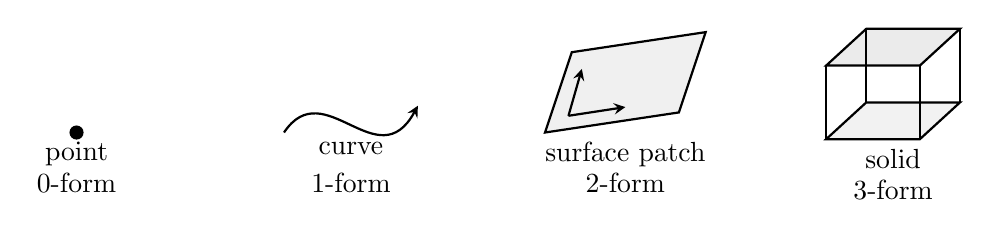
\begin{tikzpicture}[scale=0.85, >=stealth]
    \begin{scope}
        \fill (0,0) circle (3pt);
        \node[below] at (0,0) {point};
        \node at (0,-0.75) {\(0\)-form};
    \end{scope}

    \begin{scope}[shift={(3.1,0)}]
        \draw[thick, ->] (0,0) .. controls (0.6,0.9) and (1.4,-0.7) .. (2.0,0.4);
        \node[below] at (1,0) {curve};
        \node at (1,-0.75) {\(1\)-form};
    \end{scope}

    \begin{scope}[shift={(7,0)}]
        \coordinate (A) at (0,0);
        \coordinate (B) at (2,0.3);
        \coordinate (C) at (2.4,1.5);
        \coordinate (D) at (0.4,1.2);
        \draw[fill=gray!12, thick] (A)--(B)--(C)--(D)--cycle;
        \draw[->, thick] (0.35,0.25) -- (1.2,0.38);
        \draw[->, thick] (0.35,0.25) -- (0.55,0.95);
        \node[below] at (1.2,0) {surface patch};
        \node at (1.2,-0.75) {\(2\)-form};
    \end{scope}

    \begin{scope}[shift={(11.2,-0.1)}]
        \coordinate (O) at (0,0);
        \coordinate (A) at (1.4,0);
        \coordinate (B) at (2.0,0.55);
        \coordinate (C) at (0.6,0.55);
        \coordinate (D) at (0,1.1);
        \coordinate (E) at (1.4,1.1);
        \coordinate (F) at (2.0,1.65);
        \coordinate (G) at (0.6,1.65);

        \draw[fill=gray!10, thick] (O)--(A)--(B)--(C)--cycle;
        \draw[fill=gray!16, thick] (D)--(E)--(F)--(G)--cycle;
        \draw[thick] (O)--(D);
        \draw[thick] (A)--(E);
        \draw[thick] (B)--(F);
        \draw[thick] (C)--(G);

        \node[below] at (1.0,0) {solid};
        \node at (1.0,-0.75) {\(3\)-form};
    \end{scope}
\end{tikzpicture}
\caption{A \(k\)-form is built to be integrated over \(k\)-dimensional oriented objects.}
\end{figure}

This is the guiding idea:

\[
\boxed{
    \text{A differential form is an object designed to be integrated.}
}
\]

The symbols \(dx\), \(dy\), \(dz\), and their wedge products are not decorations.  They
tell the form what kind of tiny geometric piece it is measuring.

\subsection{\texorpdfstring{\(0\)}{0}-forms: functions}

A \(0\)-form is a function.

For example, on the real line,
\[
    f(x)=x^2
\]
is a \(0\)-form.  On the plane,
\[
    T(x,y)=20+\frac{6}{1+(x-2)^2+(y-1)^2}
\]
is also a \(0\)-form.  It assigns one number to each point.

The unusual part is integration.  A \(0\)-form is integrated over oriented points.  An
oriented point is just a point with a sign attached:
\[
    +P
    \qquad\text{or}\qquad
    -P.
\]
We define
\[
    \int_{+P} f=f(P),
    \qquad
    \int_{-P} f=-f(P).
\]

This may look strange until we remember the Fundamental Theorem of Calculus.  The
oriented boundary of the interval \([a,b]\) is
\[
    \partial[a,b]=\{b\}-\{a\}.
\]
So
\[
    \int_{\partial[a,b]} f
    =
    f(b)-f(a).
\]
That is exactly the boundary term in
\[
    \int_a^b f'(x)\,dx=f(b)-f(a).
\]

\begin{example}[A function on the boundary of an interval]
Let
\[
    f(x)=x^2+1
\]
and let
\[
    I=[1,4].
\]
Then
\[
    \partial I=\{4\}-\{1\}.
\]
Therefore
\[
\begin{aligned}
    \int_{\partial I} f
    &=
    f(4)-f(1)\\
    &=
    17-2\\
    &=
    15.
\end{aligned}
\]
The signs on the endpoints matter.  The right endpoint is positive, and the left
endpoint is negative.
\end{example}

This is why functions belong in the forms family.  They are the forms of degree zero.
They do not measure length, area, or volume.  They measure signed points.

\begin{definition}[\(0\)-form]
A \emph{\(0\)-form} on a region \(D\) is a scalar function
\[
    f:D\to\mathbb R.
\]
It is integrated over oriented \(0\)-dimensional objects, which are signed collections
of points.
\end{definition}

Later, the exterior derivative will turn a \(0\)-form into a \(1\)-form:
\[
    f
    \quad\longmapsto\quad
    df.
\]
That is the form version of taking a derivative.

\subsection{\texorpdfstring{\(1\)}{1}-forms: line-measuring objects}

A \(1\)-form measures one tangent direction at a time.  That is why it is integrated
along a curve.

The work form of a vector field
\[
    \mathbf F=(P,Q,R)
\]
is
\[
    \omega=P\,dx+Q\,dy+R\,dz.
\]
At each tiny step along a curve, it adds
\[
    P(\text{tiny }x\text{-change})
    +
    Q(\text{tiny }y\text{-change})
    +
    R(\text{tiny }z\text{-change}).
\]

\begin{example}[A turnstile that charges by displacement]
A robot moves across a warehouse floor.  The cost of a tiny move is
\[
    \omega=3\,dx+2\,dy.
\]
Moving east by one meter costs \(3\) units.  Moving north by one meter costs \(2\)
units.  Moving west or south gives a negative cost, because the displacement is oriented.

Let the robot move from \((0,0)\) to \((4,1)\) along the straight path
\[
    \mathbf r(t)=(4t,t),
    \qquad
    0\le t\le1.
\]
Then
\[
    dx=4\,dt,
    \qquad
    dy=dt.
\]
So
\[
\begin{aligned}
    \int_C \omega
    &=
    \int_0^1 \bigl(3(4\,dt)+2(dt)\bigr)\\
    &=
    \int_0^1 14\,dt\\
    &=
    14.
\end{aligned}
\]
The \(1\)-form did not measure how long the path was.  It measured the oriented
coordinate changes along the path.
\end{example}

\begin{definition}[\(1\)-form]
A \emph{\(1\)-form} on a region \(D\subseteq\mathbb R^2\) is an expression
\[
    \omega=P(x,y)\,dx+Q(x,y)\,dy.
\]
A \emph{\(1\)-form} on a region \(D\subseteq\mathbb R^3\) is an expression
\[
    \omega=P(x,y,z)\,dx+Q(x,y,z)\,dy+R(x,y,z)\,dz.
\]
It is integrated over oriented curves.
\end{definition}

A \(1\)-form changes sign when the orientation of the curve is reversed:
\[
    \int_{-C}\omega=-\int_C\omega.
\]
That sign is part of the object.  A \(1\)-form is not an unsigned length density like
\[
    \rho\,ds.
\]
The form \(P\,dx+Q\,dy+R\,dz\) cares which way the curve is traveled.

\subsection{\texorpdfstring{\(2\)}{2}-forms: surface-measuring objects}

A \(2\)-form measures an oriented area piece.  In the plane, the basic area form is
\[
    dx\wedge dy.
\]
So a typical \(2\)-form in the plane is
\[
    \alpha=M(x,y)\,dx\wedge dy.
\]

On a positively oriented region in the \(xy\)-plane, this acts like
\[
    M\,dA.
\]
But the wedge notation remembers the sign:
\[
    dy\wedge dx=-dx\wedge dy.
\]

\begin{example}[A signed paint layer on a floor tile]
Let
\[
    \alpha=(2+x)\,dx\wedge dy
\]
on the rectangle
\[
    R=[0,3]\times[0,2],
\]
with the usual orientation of the plane.  Then
\[
\begin{aligned}
    \int_R \alpha
    &=
    \int_0^3\int_0^2 (2+x)\,dy\,dx\\
    &=
    \int_0^3 2(2+x)\,dx\\
    &=
    \left[4x+x^2\right]_0^3\\
    &=
    21.
\end{aligned}
\]
If we reverse the orientation of \(R\), the same form gives
\[
    -21.
\]
The physical amount of paint would not become negative, but the oriented integral
does.  A \(2\)-form measures signed area.
\end{example}

In space, a surface can have shadows on three coordinate planes.  The basic \(2\)-forms
are
\[
    dy\wedge dz,\qquad dz\wedge dx,\qquad dx\wedge dy.
\]
A general \(2\)-form in space has the shape
\[
    \Phi=A\,dy\wedge dz+B\,dz\wedge dx+C\,dx\wedge dy.
\]

Flux forms are the main example:
\[
    \Phi_{\mathbf F}
    =
    P\,dy\wedge dz
    +
    Q\,dz\wedge dx
    +
    R\,dx\wedge dy
\]
for a vector field
\[
    \mathbf F=(P,Q,R).
\]

\begin{example}[Flow through a coordinate screen]
Let
\[
    \Phi=5\,dy\wedge dz+2\,dz\wedge dx.
\]
Take the screen
\[
    x=1,
    \qquad
    0\le y\le2,
    \qquad
    0\le z\le3,
\]
oriented in the positive \(x\)-direction.  A parametrization is
\[
    \mathbf r(y,z)=(1,y,z).
\]
On this screen,
\[
    dy\wedge dz
\]
is the positive area form.  Also,
\[
    dx=0,
\]
so
\[
    dz\wedge dx=0.
\]
Thus
\[
    \mathbf r^*\Phi=5\,dy\wedge dz.
\]
Therefore
\[
\begin{aligned}
    \int_S \Phi
    &=
    \int_0^2\int_0^3 5\,dz\,dy\\
    &=
    30.
\end{aligned}
\]
Only the \(dy\wedge dz\) part crosses a screen perpendicular to the \(x\)-axis.
\end{example}

\begin{definition}[\(2\)-form]
A \emph{\(2\)-form} on a region in the plane has the form
\[
    \alpha=M(x,y)\,dx\wedge dy.
\]
A \emph{\(2\)-form} on a region in space has the form
\[
    \Phi=A\,dy\wedge dz+B\,dz\wedge dx+C\,dx\wedge dy.
\]
It is integrated over oriented surfaces or oriented plane regions.
\end{definition}

Surface area integrals such as
\[
    \iint_S f\,dS
\]
do not need an orientation.  A \(2\)-form integral does.  That is why flux is the natural
surface integral for forms.

\subsection{\texorpdfstring{\(3\)}{3}-forms: volume-measuring objects}

A \(3\)-form measures oriented volume in space.  The basic volume form is
\[
    dx\wedge dy\wedge dz.
\]
A typical \(3\)-form is
\[
    \Omega=H(x,y,z)\,dx\wedge dy\wedge dz.
\]

\begin{example}[Density in a storage box]
A gas fills the box
\[
    E=[0,2]\times[0,1]\times[0,3].
\]
Suppose its density form is
\[
    \Omega=(5+z)\,dx\wedge dy\wedge dz.
\]
Using the usual orientation of space,
\[
\begin{aligned}
    \int_E \Omega
    &=
    \int_0^2\int_0^1\int_0^3 (5+z)\,dz\,dy\,dx\\
    &=
    \int_0^2\int_0^1
    \left[5z+\frac{z^2}{2}\right]_0^3
    \,dy\,dx\\
    &=
    \int_0^2\int_0^1
    \frac{39}{2}
    \,dy\,dx\\
    &=
    39.
\end{aligned}
\]
So the total mass is
\[
    39.
\]
If we reverse the orientation of space, the form integral becomes \(-39\).  For physical
mass we usually keep the standard orientation fixed and report the positive number.
\end{example}

\begin{definition}[\(3\)-form]
A \emph{\(3\)-form} on a region in space is an expression
\[
    \Omega=H(x,y,z)\,dx\wedge dy\wedge dz.
\]
It is integrated over oriented solid regions.
\end{definition}

The whole family now fits into one picture:

\[
\begin{array}{c|c|c|c}
\text{Degree} & \text{Typical form} & \text{Tiny object measured} & \text{Integral} \\ \hline
0 & f & \text{oriented point} & \int_{\partial I} f\\[1mm]
1 & P\,dx+Q\,dy+R\,dz & \text{oriented tangent vector} & \int_C \omega\\[1mm]
2 & A\,dy\wedge dz+B\,dz\wedge dx+C\,dx\wedge dy
& \text{oriented parallelogram} & \int_S \Phi\\[1mm]
3 & H\,dx\wedge dy\wedge dz & \text{oriented box} & \int_E \Omega
\end{array}
\]

The table hides one important question.  A \(1\)-form is built from \(dx\), \(dy\), and
\(dz\).  But what are these symbols really?  They are not tiny numbers.  They are
linear measuring rules for tangent vectors.  Giving those rules their proper name,
\emph{covectors}, is the next step.

\section{Covectors and differentials}
\label{sec:16.2}

Section \ref{sec:16.1} treated forms as integrands.  A \(1\)-form measures tiny tangent
arrows along a curve, and a \(2\)-form measures tiny oriented parallelograms on a
surface.  To understand the pieces of those forms, we start with the simplest question:
what does \(dx\) do to a vector?

\subsection{Linear functions on vectors}

Stand on a flat loading dock.  A small cart can move east, north, and up.  Write one
displacement as
\[
    \mathbf v=(v_x,v_y,v_z).
\]
Suppose a scanner assigns the number
\[
    L(\mathbf v)=4v_x-v_y+2v_z
\]
to that displacement.  A move one meter east counts \(4\).  A move one meter north
counts \(-1\).  A move one meter upward counts \(2\).

This scanner is linear.  If the cart makes two displacements,
\[
    \mathbf u
    \qquad\text{and}\qquad
    \mathbf v,
\]
then
\[
    L(\mathbf u+\mathbf v)=L(\mathbf u)+L(\mathbf v).
\]
If the displacement is doubled, the reading doubles:
\[
    L(2\mathbf v)=2L(\mathbf v).
\]

For example, let
\[
    \mathbf u=(1,3,0),
    \qquad
    \mathbf v=(2,-1,4).
\]
Then
\[
    L(\mathbf u)=4(1)-3+0=1
\]
and
\[
    L(\mathbf v)=4(2)-(-1)+2(4)=17.
\]
Also,
\[
    \mathbf u+\mathbf v=(3,2,4),
\]
so
\[
    L(\mathbf u+\mathbf v)=4(3)-2+2(4)=18.
\]
Indeed,
\[
    18=1+17.
\]

This is the kind of object hiding behind \(dx\), \(dy\), and \(dz\).

\begin{definition}[Covector]
A \emph{covector} at a point is a linear function that takes a tangent vector at that
point and returns a number.

In \(\mathbb R^3\), a covector has the form
\[
    a\,dx+b\,dy+c\,dz
\]
at a point, and it acts on
\[
    \mathbf v=(v_x,v_y,v_z)
\]
by
\[
\boxed{
    (a\,dx+b\,dy+c\,dz)(\mathbf v)
    =
    av_x+bv_y+cv_z.
}
\]
\end{definition}

A vector points.  A covector measures.

They are related, especially when a dot product is available, but they are not the same
kind of object.

\subsection{\texorpdfstring{\(dx\), \(dy\), and \(dz\)}{dx, dy, and dz} as coordinate covectors}

The coordinate covectors are the simplest measuring rules:
\[
    dx(\mathbf v)=v_x,
\]
\[
    dy(\mathbf v)=v_y,
\]
\[
    dz(\mathbf v)=v_z.
\]
They read the coordinate components of a tangent vector.

\begin{figure}[h]
\centering
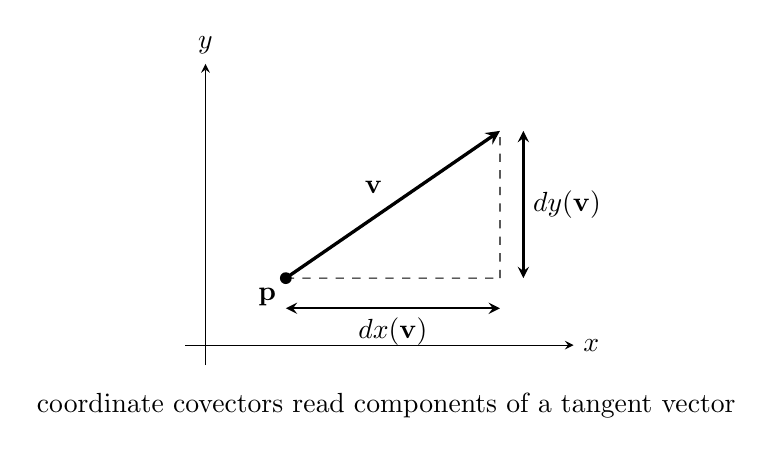
\begin{tikzpicture}[scale=0.85, >=stealth]
    \draw[->] (-0.3,0) -- (5.5,0) node[right] {\(x\)};
    \draw[->] (0,-0.3) -- (0,4.2) node[above] {\(y\)};

    \coordinate (P) at (1.2,1.0);
    \coordinate (Q) at (4.4,3.2);

    \fill (P) circle (2.5pt);
    \node[below left] at (P) {\(\mathbf p\)};

    \draw[->, very thick] (P) -- (Q) node[midway, above left] {\(\mathbf v\)};

    \draw[dashed] (P) -- (4.4,1.0);
    \draw[dashed] (4.4,1.0) -- (Q);

    \draw[<->, thick] (1.2,0.55) -- (4.4,0.55);
    \node[below] at (2.8,0.55) {\(dx(\mathbf v)\)};

    \draw[<->, thick] (4.75,1.0) -- (4.75,3.2);
    \node[right] at (4.75,2.1) {\(dy(\mathbf v)\)};

    \node at (2.7,-0.9) {coordinate covectors read components of a tangent vector};
\end{tikzpicture}
\caption{\(dx\) reads the horizontal component, and \(dy\) reads the vertical component.}
\end{figure}

For instance, if
\[
    \mathbf v=(3,-5,2),
\]
then
\[
    dx(\mathbf v)=3,
    \qquad
    dy(\mathbf v)=-5,
    \qquad
    dz(\mathbf v)=2.
\]

A general covector is a linear combination of these coordinate covectors.

\begin{example}[A covector from its coordinate readings]
Let
\[
    \eta=4\,dx-dy+2\,dz.
\]
Then on
\[
    \mathbf v=(3,-5,2),
\]
we get
\[
\begin{aligned}
    \eta(\mathbf v)
    &=
    4\,dx(\mathbf v)-dy(\mathbf v)+2\,dz(\mathbf v)\\
    &=
    4(3)-(-5)+2(2)\\
    &=
    21.
\end{aligned}
\]
\end{example}

The next theorem is the covector version of a familiar fact: a linear rule is determined
by what it does to the standard basis vectors.

\begin{theorem}[Every covector is a linear combination of coordinate covectors]
Let \(\eta\) be a covector in \(\mathbb R^3\).  Then there are unique numbers
\(a,b,c\) such that
\[
\boxed{
    \eta=a\,dx+b\,dy+c\,dz.
}
\]
The coefficients are
\[
\boxed{
    a=\eta(\mathbf i),
    \qquad
    b=\eta(\mathbf j),
    \qquad
    c=\eta(\mathbf k).
}
\]
\end{theorem}

\begin{proof}
Every vector
\[
    \mathbf v=(v_x,v_y,v_z)
\]
can be written as
\[
    \mathbf v=v_x\mathbf i+v_y\mathbf j+v_z\mathbf k.
\]
Since \(\eta\) is linear,
\[
\begin{aligned}
    \eta(\mathbf v)
    &=
    v_x\eta(\mathbf i)+v_y\eta(\mathbf j)+v_z\eta(\mathbf k).
\end{aligned}
\]
Let
\[
    a=\eta(\mathbf i),
    \qquad
    b=\eta(\mathbf j),
    \qquad
    c=\eta(\mathbf k).
\]
Then
\[
    \eta(\mathbf v)=av_x+bv_y+cv_z.
\]
But this is exactly
\[
    (a\,dx+b\,dy+c\,dz)(\mathbf v).
\]
The coefficients are unique because applying the covector to \(\mathbf i,\mathbf j\),
and \(\mathbf k\) forces them.
\end{proof}

In the plane, the same statement says every covector has the form
\[
    a\,dx+b\,dy.
\]

\subsection{Evaluating a \texorpdfstring{\(1\)}{1}-form on a tangent vector}

A covector lives at one point.  A \(1\)-form is a covector field: it attaches a covector
to every point.

For example,
\[
    \omega=(x+y)\,dx+x\,dy+z\,dz
\]
is a \(1\)-form in space.  At the point
\[
    \mathbf p=(2,1,-1),
\]
its coefficients become
\[
    x+y=3,
    \qquad
    x=2,
    \qquad
    z=-1.
\]
So at that point,
\[
    \omega_{\mathbf p}=3\,dx+2\,dy-dz.
\]

Now evaluate it on the tangent vector
\[
    \mathbf v=(3,-4,2).
\]
We get
\[
\begin{aligned}
    \omega_{\mathbf p}(\mathbf v)
    &=
    3\,dx(\mathbf v)+2\,dy(\mathbf v)-dz(\mathbf v)\\
    &=
    3(3)+2(-4)-2\\
    &=
    -1.
\end{aligned}
\]

The subscript matters:
\[
    \omega_{\mathbf p}
\]
means the covector obtained by freezing the coefficient functions at the point
\(\mathbf p\).

\begin{definition}[Evaluating a \(1\)-form]
Let
\[
    \omega=P\,dx+Q\,dy+R\,dz
\]
be a \(1\)-form on a region in space.  At a point \(\mathbf p\), and on a tangent vector
\[
    \mathbf v=(v_x,v_y,v_z),
\]
we define
\[
\boxed{
    \omega_{\mathbf p}(\mathbf v)
    =
    P(\mathbf p)v_x+Q(\mathbf p)v_y+R(\mathbf p)v_z.
}
\]
\end{definition}

This is the local measurement behind every line integral.

If a curve is
\[
    \mathbf r(t),
\]
then its tangent vector is
\[
    \mathbf r'(t).
\]
At time \(t\), the \(1\)-form measures that tangent vector:
\[
    \omega_{\mathbf r(t)}(\mathbf r'(t)).
\]
The line integral is obtained by adding those measurements over time:
\[
\boxed{
    \int_C \omega
    =
    \int_a^b
    \omega_{\mathbf r(t)}(\mathbf r'(t))\,dt.
}
\]

\begin{example}[A form along a circular path]
Let
\[
    \omega=-y\,dx+x\,dy
\]
and let
\[
    \mathbf r(t)=(\cos t,\sin t),
    \qquad
    0\le t\le2\pi.
\]
Then
\[
    \mathbf r'(t)=(-\sin t,\cos t).
\]
At the point
\[
    \mathbf r(t),
\]
the form is
\[
    \omega_{\mathbf r(t)}
    =
    -\sin t\,dx+\cos t\,dy.
\]
Evaluate on the tangent vector:
\[
\begin{aligned}
    \omega_{\mathbf r(t)}(\mathbf r'(t))
    &=
    (-\sin t)(-\sin t)+(\cos t)(\cos t)\\
    &=
    1.
\end{aligned}
\]
Therefore
\[
    \int_C \omega
    =
    \int_0^{2\pi}1\,dt
    =
    2\pi.
\]
The form gives \(1\) on the counterclockwise unit tangent all the way around the circle.
\end{example}

This language separates two jobs.  The curve supplies tangent vectors.  The form
measures them.

\subsection{Why gradients require a dot product but differentials do not}

The differential of a function is a covector.

Let
\[
    f(x,y,z)
\]
be differentiable at a point
\[
    \mathbf p=(a,b,c).
\]
The best linear prediction for the change in \(f\) is
\[
    df_{\mathbf p}
    =
    f_x(\mathbf p)\,dx
    +
    f_y(\mathbf p)\,dy
    +
    f_z(\mathbf p)\,dz.
\]
On a tangent vector
\[
    \mathbf v=(v_x,v_y,v_z),
\]
this gives
\[
\boxed{
    df_{\mathbf p}(\mathbf v)
    =
    f_x(\mathbf p)v_x
    +
    f_y(\mathbf p)v_y
    +
    f_z(\mathbf p)v_z.
}
\]

This formula does not mention length or angle.  It only uses how the function changes
under a displacement.

The gradient vector appears when we use the usual Euclidean dot product.  With that
dot product,
\[
    \nabla f(\mathbf p)
    =
    \bigl(f_x(\mathbf p),f_y(\mathbf p),f_z(\mathbf p)\bigr),
\]
and
\[
\boxed{
    df_{\mathbf p}(\mathbf v)
    =
    \nabla f(\mathbf p)\cdot\mathbf v.
}
\]

\begin{theorem}[The differential is represented by the gradient in Euclidean space]
Let \(f\) be differentiable at \(\mathbf p\in\mathbb R^3\), and use the usual dot product.
Then the covector \(df_{\mathbf p}\) is represented by the gradient vector:
\[
\boxed{
    df_{\mathbf p}(\mathbf v)=\nabla f(\mathbf p)\cdot\mathbf v
}
\]
for every tangent vector \(\mathbf v\).
\end{theorem}

\begin{proof}
Write
\[
    \mathbf v=(v_x,v_y,v_z).
\]
By the definition of \(df_{\mathbf p}\),
\[
    df_{\mathbf p}(\mathbf v)
    =
    f_x(\mathbf p)v_x
    +
    f_y(\mathbf p)v_y
    +
    f_z(\mathbf p)v_z.
\]
By the definition of the usual dot product,
\[
    \nabla f(\mathbf p)\cdot\mathbf v
    =
    \bigl(f_x(\mathbf p),f_y(\mathbf p),f_z(\mathbf p)\bigr)
    \cdot
    (v_x,v_y,v_z),
\]
which is the same expression.
\end{proof}

The phrase ``use the usual dot product'' is doing real work.

\begin{example}[The same differential can have different gradient vectors]
Take the function
\[
    f(x,y)=3x+4y.
\]
Its differential is
\[
\boxed{
    df=3\,dx+4\,dy.
}
\]
This covector is fixed.  On a vector
\[
    \mathbf v=(v_x,v_y),
\]
it gives
\[
    df(\mathbf v)=3v_x+4v_y.
\]

With the usual dot product,
\[
    (a,b)\cdot(v_x,v_y)=av_x+bv_y,
\]
the representing gradient vector is
\[
    \nabla f=(3,4).
\]

Now change only the dot product.  Suppose the geometry of the floor measures vertical
motion with four times the weight:
\[
    \langle (a,b),(v_x,v_y)\rangle_*
    =
    av_x+4bv_y.
\]
The same differential
\[
    df=3\,dx+4\,dy
\]
is now represented by the vector
\[
    \mathbf g=(3,1),
\]
because
\[
    \langle (3,1),(v_x,v_y)\rangle_*
    =
    3v_x+4v_y
    =
    df(\mathbf v).
\]

So the differential did not change:
\[
    df=3\,dx+4\,dy.
\]
The gradient vector changed because the dot product changed.
\end{example}

This is the moral:

\[
\boxed{
    df \text{ is a covector.  The gradient is the vector that represents } df
    \text{ after a dot product is chosen.}
}
\]

In ordinary Euclidean coordinates, the distinction is easy to miss because
\[
    df=f_x\,dx+f_y\,dy+f_z\,dz
\]
and
\[
    \nabla f=(f_x,f_y,f_z)
\]
use the same coefficients.  But they have different jobs.  The differential measures
tangent vectors directly.  The gradient is a vector chosen so that the dot product with
a tangent vector gives the same measurement.

This distinction becomes more valuable as soon as we multiply covectors.  A single
covector measures one direction.  To measure an oriented parallelogram, we need two
directions at once.  The operation that combines covectors into area-measuring forms
is the wedge product.
% =====================================================================
%  Chapter 16: Differential Forms and the Wedge Product
%  Sections 16.3 and 16.4
% =====================================================================

\section{The wedge product}
\label{sec:16.3}

Section \ref{sec:16.2} ended with covectors.  A covector measures one tangent vector.
But a surface patch gives two tangent vectors, and a tiny box gives three.  To measure
oriented area and oriented volume, we need a way to combine covectors.

That way is the wedge product.

\subsection{Oriented area from two covectors}

Start with a small parallelogram in the plane.  Its first edge is
\[
    \mathbf u=(3,1),
\]
and its second edge is
\[
    \mathbf v=(1,4).
\]
The ordered pair
\[
    (\mathbf u,\mathbf v)
\]
means that we travel first in the \(\mathbf u\)-direction and then in the
\(\mathbf v\)-direction.  That order gives the parallelogram an orientation.

\begin{figure}[h]
\centering
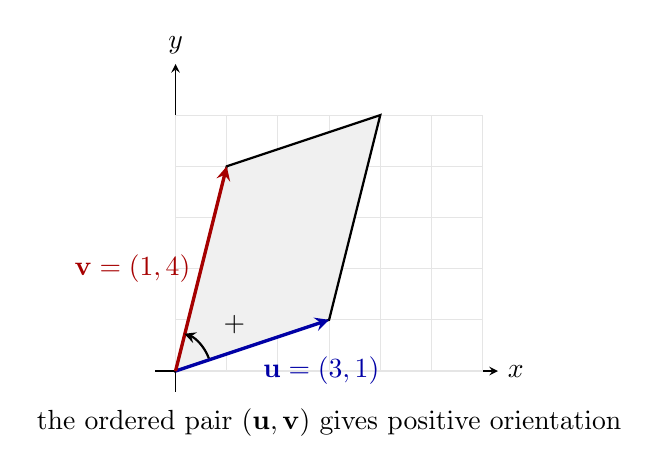
\begin{tikzpicture}[scale=0.65, >=stealth]
    \draw[->] (-0.4,0) -- (6.3,0) node[right] {\(x\)};
    \draw[->] (0,-0.4) -- (0,6.0) node[above] {\(y\)};

    \draw[gray!20, step=1] (0,0) grid (6,5);

    \coordinate (O) at (0,0);
    \coordinate (U) at (3,1);
    \coordinate (V) at (1,4);
    \coordinate (UV) at (4,5);

    \draw[fill=gray!12, thick] (O)--(U)--(UV)--(V)--cycle;

    \draw[->, very thick, blue!65!black] (O)--(U)
        node[midway, below right] {\(\mathbf u=(3,1)\)};
    \draw[->, very thick, red!65!black] (O)--(V)
        node[midway, left] {\(\mathbf v=(1,4)\)};

    \draw[dashed] (U)--(UV);
    \draw[dashed] (V)--(UV);

    \draw[->, thick] (0.65,0.25) arc[start angle=20,end angle=70,radius=0.8];
    \node at (1.15,0.9) {\(+\)};

    \node at (3,-1.0) {the ordered pair \((\mathbf u,\mathbf v)\) gives positive orientation};
\end{tikzpicture}
\caption{The signed area of a parallelogram depends on the order of its two edge vectors.}
\end{figure}

The signed area is the determinant
\[
    \begin{vmatrix}
        3&1\\
        1&4
    \end{vmatrix}
    =
    3\cdot4-1\cdot1
    =
    11.
\]
Now write the same computation using the coordinate covectors
\[
    dx,\qquad dy.
\]
They read components:
\[
    dx(\mathbf u)=3,
    \qquad
    dy(\mathbf u)=1,
\]
and
\[
    dx(\mathbf v)=1,
    \qquad
    dy(\mathbf v)=4.
\]
The signed area is
\[
    dx(\mathbf u)dy(\mathbf v)-dx(\mathbf v)dy(\mathbf u).
\]
For our two vectors, this gives
\[
    3\cdot4-1\cdot1=11.
\]

This expression is so common that we give it its own symbol:
\[
\boxed{
    (dx\wedge dy)(\mathbf u,\mathbf v)
    =
    dx(\mathbf u)dy(\mathbf v)-dx(\mathbf v)dy(\mathbf u).
}
\]

The symbol
\[
    dx\wedge dy
\]
is the basic oriented area form in the \(xy\)-plane.  It eats two tangent vectors and
returns their signed \(xy\)-area.

\begin{example}[The same parallelogram with reversed order]
Use the same vectors
\[
    \mathbf u=(3,1),
    \qquad
    \mathbf v=(1,4),
\]
but feed them to \(dx\wedge dy\) in the opposite order:
\[
\begin{aligned}
    (dx\wedge dy)(\mathbf v,\mathbf u)
    &=
    dx(\mathbf v)dy(\mathbf u)-dx(\mathbf u)dy(\mathbf v)\\
    &=
    1\cdot1-3\cdot4\\
    &=
    -11.
\end{aligned}
\]
The geometric parallelogram is the same size, but its orientation has been reversed.
\end{example}

This example contains the whole idea.  The wedge product is built to measure oriented
parallelograms.

\begin{definition}[Wedge product of two covectors]
Let \(\alpha\) and \(\beta\) be covectors at a point.  Their wedge product
\[
    \alpha\wedge\beta
\]
is the rule that takes an ordered pair of tangent vectors \((\mathbf u,\mathbf v)\) and
returns
\[
\boxed{
    (\alpha\wedge\beta)(\mathbf u,\mathbf v)
    =
    \alpha(\mathbf u)\beta(\mathbf v)
    -
    \alpha(\mathbf v)\beta(\mathbf u).
}
\]
\end{definition}

The two terms are the two possible ways to match the covectors with the two vectors.
The minus sign is what remembers orientation.

\begin{example}[A wedge product that measures a slanted coordinate area]
Let
\[
    \alpha=2\,dx+dy,
    \qquad
    \beta=dx+3\,dy.
\]
Use the vectors
\[
    \mathbf u=(1,2),
    \qquad
    \mathbf v=(4,-1).
\]
First evaluate the covectors:
\[
    \alpha(\mathbf u)=2(1)+2=4,
    \qquad
    \alpha(\mathbf v)=2(4)-1=7,
\]
and
\[
    \beta(\mathbf u)=1+3(2)=7,
    \qquad
    \beta(\mathbf v)=4+3(-1)=1.
\]
Therefore
\[
\begin{aligned}
    (\alpha\wedge\beta)(\mathbf u,\mathbf v)
    &=
    \alpha(\mathbf u)\beta(\mathbf v)
    -
    \alpha(\mathbf v)\beta(\mathbf u)\\
    &=
    4\cdot1-7\cdot7\\
    &=
    -45.
\end{aligned}
\]
The negative sign says that the ordered measurements \(\alpha,\beta\) see the ordered
vectors \(\mathbf u,\mathbf v\) with the opposite orientation.
\end{example}

A \(1\)-form measures one vector.  A wedge of two \(1\)-forms measures two vectors at
once.  That is why it becomes a \(2\)-form.

\subsection{\texorpdfstring{Antisymmetry: \(dx\wedge dy=-dy\wedge dx\)}
{Antisymmetry: dx wedge dy = - dy wedge dx}}

The wedge product changes sign when its factors are swapped.  Check this directly:
\[
\begin{aligned}
    (\beta\wedge\alpha)(\mathbf u,\mathbf v)
    &=
    \beta(\mathbf u)\alpha(\mathbf v)
    -
    \beta(\mathbf v)\alpha(\mathbf u)\\
    &=
    -\left[
    \alpha(\mathbf u)\beta(\mathbf v)
    -
    \alpha(\mathbf v)\beta(\mathbf u)
    \right].
\end{aligned}
\]
So
\[
\boxed{
    \beta\wedge\alpha=-\alpha\wedge\beta.
}
\]

For the coordinate covectors, this gives
\[
\boxed{
    dy\wedge dx=-dx\wedge dy.
}
\]
Equivalently,
\[
\boxed{
    dx\wedge dy=-dy\wedge dx.
}
\]

\begin{example}[The same area measured with \(dy\wedge dx\)]
Return again to
\[
    \mathbf u=(3,1),
    \qquad
    \mathbf v=(1,4).
\]
Then
\[
\begin{aligned}
    (dy\wedge dx)(\mathbf u,\mathbf v)
    &=
    dy(\mathbf u)dx(\mathbf v)-dy(\mathbf v)dx(\mathbf u)\\
    &=
    1\cdot1-4\cdot3\\
    &=
    -11.
\end{aligned}
\]
But
\[
    (dx\wedge dy)(\mathbf u,\mathbf v)=11.
\]
So
\[
    dy\wedge dx
\]
measures the same area with the opposite orientation.
\end{example}

This is the first algebra rule of wedge products:

\[
\boxed{
    \text{Swapping two \(1\)-forms changes the sign.}
}
\]

That sign is not a bookkeeping trick.  It is the algebraic form of a geometric fact:
swapping the two edge directions of a parallelogram reverses its orientation.

\subsection{\texorpdfstring{Why \(dx\wedge dx=0\)}{Why dx wedge dx = 0}}

Now try to wedge a covector with itself:
\[
    dx\wedge dx.
\]
For two tangent vectors \(\mathbf u\) and \(\mathbf v\),
\[
\begin{aligned}
    (dx\wedge dx)(\mathbf u,\mathbf v)
    &=
    dx(\mathbf u)dx(\mathbf v)
    -
    dx(\mathbf v)dx(\mathbf u)\\
    &=
    0.
\end{aligned}
\]
Therefore
\[
\boxed{
    dx\wedge dx=0.
}
\]
The same calculation gives
\[
\boxed{
    dy\wedge dy=0,
    \qquad
    dz\wedge dz=0.
}
\]

The geometry is simple.  A single coordinate reading repeated twice cannot measure
area.  Area needs two independent directions of measurement.  Measuring the
\(x\)-component twice collapses the picture onto one line.

More generally,
\[
\boxed{
    \alpha\wedge\alpha=0
}
\]
for every covector \(\alpha\).

\begin{example}[Parallel edge vectors give zero area]
Let
\[
    \mathbf u=(2,1),
    \qquad
    \mathbf v=(6,3).
\]
The second vector is
\[
    \mathbf v=3\mathbf u.
\]
The parallelogram has collapsed to a line segment, so its signed area should be \(0\).
Indeed,
\[
\begin{aligned}
    (dx\wedge dy)(\mathbf u,\mathbf v)
    &=
    2\cdot3-6\cdot1\\
    &=
    0.
\end{aligned}
\]
The wedge product automatically detects the collapse.
\end{example}

This is one reason wedge notation is so useful.  The rules
\[
    dx\wedge dx=0
\]
and
\[
    dx\wedge dy=-dy\wedge dx
\]
make repeated or reversed directions behave exactly as oriented area says they should.

\subsection{Building \texorpdfstring{\(2\)}{2}-forms and
\texorpdfstring{\(3\)}{3}-forms}

In the plane, there is only one basic oriented area form:
\[
    dx\wedge dy.
\]
So every \(2\)-form in the plane has the shape
\[
    M(x,y)\,dx\wedge dy.
\]

In space, a small surface patch can cast shadows on three coordinate planes.  That is
why three basic \(2\)-forms appear:
\[
    dy\wedge dz,\qquad dz\wedge dx,\qquad dx\wedge dy.
\]
Each one measures a signed shadow.

Let
\[
    \mathbf u=(u_x,u_y,u_z),
    \qquad
    \mathbf v=(v_x,v_y,v_z).
\]
Then
\[
\boxed{
    (dy\wedge dz)(\mathbf u,\mathbf v)
    =
    u_yv_z-v_yu_z,
}
\]
\[
\boxed{
    (dz\wedge dx)(\mathbf u,\mathbf v)
    =
    u_zv_x-v_zu_x,
}
\]
and
\[
\boxed{
    (dx\wedge dy)(\mathbf u,\mathbf v)
    =
    u_xv_y-v_xu_y.
}
\]
These are the signed areas of the shadows on the \(yz\)-plane, the \(zx\)-plane, and
the \(xy\)-plane.

A general \(2\)-form in space is
\[
\boxed{
    \Phi=A\,dy\wedge dz+B\,dz\wedge dx+C\,dx\wedge dy.
}
\]
It measures a weighted combination of those three signed shadows.

\begin{example}[A \(2\)-form measuring a tilted surface patch]
Suppose a small surface patch has tangent edge vectors
\[
    \mathbf u=(1,2,0),
    \qquad
    \mathbf v=(0,1,3).
\]
Compute the three coordinate shadow areas:
\[
\begin{aligned}
    (dy\wedge dz)(\mathbf u,\mathbf v)
    &=
    2\cdot3-1\cdot0
    =
    6,\\
    (dz\wedge dx)(\mathbf u,\mathbf v)
    &=
    0\cdot0-3\cdot1
    =
    -3,\\
    (dx\wedge dy)(\mathbf u,\mathbf v)
    &=
    1\cdot1-0\cdot2
    =
    1.
\end{aligned}
\]
Now let
\[
    \Phi=2\,dy\wedge dz-dz\wedge dx+4\,dx\wedge dy.
\]
Then
\[
\begin{aligned}
    \Phi(\mathbf u,\mathbf v)
    &=
    2(6)-(-3)+4(1)\\
    &=
    19.
\end{aligned}
\]
The form did not measure ordinary surface area.  It measured an oriented combination
of coordinate-plane shadows.
\end{example}

A \(3\)-form measures an oriented box.  The basic one in space is
\[
    dx\wedge dy\wedge dz.
\]
It eats three tangent vectors and returns the signed volume of the parallelepiped they
span.

If
\[
    \mathbf u,\qquad \mathbf v,\qquad \mathbf w
\]
are tangent vectors in space, then
\[
\boxed{
    (dx\wedge dy\wedge dz)(\mathbf u,\mathbf v,\mathbf w)
    =
    \det
    \begin{pmatrix}
        dx(\mathbf u)&dx(\mathbf v)&dx(\mathbf w)\\
        dy(\mathbf u)&dy(\mathbf v)&dy(\mathbf w)\\
        dz(\mathbf u)&dz(\mathbf v)&dz(\mathbf w)
    \end{pmatrix}.
}
\]
Since \(dx,dy,dz\) read the coordinate components, this is the usual determinant with
columns \(\mathbf u,\mathbf v,\mathbf w\).

\begin{example}[A \(3\)-form measuring volume]
Let
\[
    \mathbf u=(1,0,0),
    \qquad
    \mathbf v=(1,2,0),
    \qquad
    \mathbf w=(0,1,3).
\]
Then
\[
\begin{aligned}
    (dx\wedge dy\wedge dz)(\mathbf u,\mathbf v,\mathbf w)
    &=
    \det
    \begin{pmatrix}
        1&1&0\\
        0&2&1\\
        0&0&3
    \end{pmatrix}\\
    &=
    6.
\end{aligned}
\]
So the oriented volume of the box spanned by these three ordered vectors is \(6\).
If we swap \(\mathbf u\) and \(\mathbf v\), the value becomes \(-6\).
\end{example}

In space, every \(3\)-form has the shape
\[
\boxed{
    H(x,y,z)\,dx\wedge dy\wedge dz.
}
\]
There are no nonzero \(4\)-forms in ordinary three-dimensional space.  Four tangent
vectors in \(\mathbb R^3\) must be linearly dependent, so any oriented \(4\)-dimensional
volume collapses.

\subsection{Determinants as wedge-product coefficients}

The wedge product explains why determinants keep appearing in multivariable calculus.
They are the coefficients of oriented area and oriented volume.

Start in the plane.  Let
\[
    \alpha=a\,dx+b\,dy,
    \qquad
    \beta=c\,dx+d\,dy.
\]
Then
\[
\begin{aligned}
    \alpha\wedge\beta
    &=
    (a\,dx+b\,dy)\wedge(c\,dx+d\,dy)\\
    &=
    ac\,dx\wedge dx
    +ad\,dx\wedge dy
    +bc\,dy\wedge dx
    +bd\,dy\wedge dy.
\end{aligned}
\]
Now use
\[
    dx\wedge dx=0,
    \qquad
    dy\wedge dy=0,
\]
and
\[
    dy\wedge dx=-dx\wedge dy.
\]
The result is
\[
\boxed{
    \alpha\wedge\beta=(ad-bc)\,dx\wedge dy.
}
\]
The coefficient
\[
    ad-bc
\]
is a \(2\times2\) determinant:
\[
\boxed{
    ad-bc
    =
    \begin{vmatrix}
        a&b\\
        c&d
    \end{vmatrix}.
}
\]

\begin{example}[The determinant inside a wedge product]
Let
\[
    \alpha=2\,dx+dy,
    \qquad
    \beta=dx+4\,dy.
\]
Then
\[
\begin{aligned}
    \alpha\wedge\beta
    &=
    (2\cdot4-1\cdot1)\,dx\wedge dy\\
    &=
    7\,dx\wedge dy.
\end{aligned}
\]
The number \(7\) is the signed area scale factor hidden in the two covectors.
\end{example}

In space, wedge two \(1\)-forms:
\[
    \alpha=a\,dx+b\,dy+c\,dz,
\]
and
\[
    \beta=p\,dx+q\,dy+r\,dz.
\]
A direct expansion gives
\[
\boxed{
    \alpha\wedge\beta
    =
    (br-cq)\,dy\wedge dz
    +
    (cp-ar)\,dz\wedge dx
    +
    (aq-bp)\,dx\wedge dy.
}
\]
The three coefficients are the components of the cross product of the coefficient
vectors:
\[
    (a,b,c)\times(p,q,r)
    =
    (br-cq,\ cp-ar,\ aq-bp).
\]
So the cross product is also hiding inside the wedge product.  The wedge product keeps
the result as a \(2\)-form, while the cross product turns the same coefficients into a
vector.

For three \(1\)-forms,
\[
    \alpha=a\,dx+b\,dy+c\,dz,
\]
\[
    \beta=p\,dx+q\,dy+r\,dz,
\]
and
\[
    \gamma=m\,dx+n\,dy+s\,dz,
\]
the wedge product is
\[
\boxed{
    \alpha\wedge\beta\wedge\gamma
    =
    \begin{vmatrix}
        a&b&c\\
        p&q&r\\
        m&n&s
    \end{vmatrix}
    dx\wedge dy\wedge dz.
}
\]

\begin{example}[A triple wedge product]
Let
\[
    \alpha=dx+dy,
    \qquad
    \beta=2\,dy+dz,
    \qquad
    \gamma=3\,dx-dz.
\]
Then
\[
    \alpha\wedge\beta\wedge\gamma
    =
    \begin{vmatrix}
        1&1&0\\
        0&2&1\\
        3&0&-1
    \end{vmatrix}
    dx\wedge dy\wedge dz.
\]
Compute the determinant:
\[
\begin{aligned}
    \begin{vmatrix}
        1&1&0\\
        0&2&1\\
        3&0&-1
    \end{vmatrix}
    &=
    1(2(-1)-1\cdot0)
    -
    1(0(-1)-1\cdot3)\\
    &=
    -2-(-3)\\
    &=
    1.
\end{aligned}
\]
So
\[
\boxed{
    \alpha\wedge\beta\wedge\gamma
    =
    dx\wedge dy\wedge dz.
}
\]
\end{example}

The wedge product has now given us the basic measuring objects.  But forms in real
integrals do not usually have constant coefficients.  They have functions attached to
them, and we need to add them, scale them, and multiply them without losing track of
degree.  That is the algebra of forms.

\section{Algebra of forms}
\label{sec:16.4}

The wedge product gives the multiplication rule.  Now we need the everyday algebra:
adding forms, multiplying them by functions, and keeping signs straight.  The main
rule is simple: the degree tells us what kind of object the form measures, so the degree
must be respected.

\subsection{Adding forms of the same degree}

Two \(1\)-forms can be added because both measure tangent vectors.  For example,
\[
    \omega_1=3\,dx-y\,dy
\]
and
\[
    \omega_2=x\,dx+2\,dy
\]
combine to make
\[
\begin{aligned}
    \omega_1+\omega_2
    &=
    (3\,dx-y\,dy)+(x\,dx+2\,dy)\\
    &=
    (x+3)\,dx+(2-y)\,dy.
\end{aligned}
\]
On any tangent vector, the new form gives the sum of the two old readings.

\begin{example}[Two small meters along a path]
A cart moves in the plane.  One meter charges
\[
    \omega_1=2\,dx+dy,
\]
and another charges
\[
    \omega_2=-dx+4\,dy.
\]
Together they charge
\[
    \omega_1+\omega_2=dx+5\,dy.
\]
If the cart has tangent vector
\[
    \mathbf v=(3,-1),
\]
then
\[
    \omega_1(\mathbf v)=2(3)+(-1)=5,
\]
and
\[
    \omega_2(\mathbf v)=-3+4(-1)=-7.
\]
The combined reading is
\[
    5+(-7)=-2.
\]
Using the combined form directly,
\[
    (dx+5\,dy)(\mathbf v)=3+5(-1)=-2.
\]
\end{example}

The same rule works for \(2\)-forms.  In space,
\[
    \Phi_1=A_1\,dy\wedge dz+B_1\,dz\wedge dx+C_1\,dx\wedge dy
\]
and
\[
    \Phi_2=A_2\,dy\wedge dz+B_2\,dz\wedge dx+C_2\,dx\wedge dy
\]
add to
\[
\boxed{
    \Phi_1+\Phi_2
    =
    (A_1+A_2)\,dy\wedge dz
    +(B_1+B_2)\,dz\wedge dx
    +(C_1+C_2)\,dx\wedge dy.
}
\]
Two \(3\)-forms add in the same way:
\[
    H_1\,dx\wedge dy\wedge dz
    +
    H_2\,dx\wedge dy\wedge dz
    =
    (H_1+H_2)\,dx\wedge dy\wedge dz.
\]

We do not add a \(1\)-form and a \(2\)-form as a single form in this book.  They measure
different kinds of objects.  The expression
\[
    dx+dx\wedge dy
\]
contains a line-measuring part and an area-measuring part.  Advanced books allow such
mixed objects, but here we keep each degree separate.

\begin{definition}[Addition of forms]
Forms of the same degree are added coefficient by coefficient.  The sum has the same
degree.
\end{definition}

\subsection{Multiplying forms by functions}

A function is a \(0\)-form.  It assigns a number to each point.  Multiplying a form by a
function scales the form point by point.

For example, if
\[
    \omega=dx+2\,dy
\]
and
\[
    f(x,y)=1+x^2,
\]
then
\[
\boxed{
    f\omega=(1+x^2)\,dx+2(1+x^2)\,dy.
}
\]
At the point \((2,1)\), the scaling factor is
\[
    f(2,1)=5.
\]
So at that point,
\[
    (f\omega)_{(2,1)}=5\,dx+10\,dy.
\]

\begin{example}[A position-dependent toll]
A robot moves across a warehouse floor.  The basic motion charge is
\[
    \omega=3\,dx+dy.
\]
Near a loading area, the cost is multiplied by
\[
    f(x,y)=1+\frac{x}{10}.
\]
The actual cost form is
\[
    f\omega
    =
    \left(1+\frac{x}{10}\right)(3\,dx+dy).
\]
So
\[
    f\omega
    =
    \left(3+\frac{3x}{10}\right)dx
    +
    \left(1+\frac{x}{10}\right)dy.
\]
At \(x=0\), the original cost is unchanged.  At \(x=10\), the whole form is doubled.
\end{example}

For \(2\)-forms,
\[
    f\left(A\,dy\wedge dz+B\,dz\wedge dx+C\,dx\wedge dy\right)
\]
means
\[
\boxed{
    fA\,dy\wedge dz+fB\,dz\wedge dx+fC\,dx\wedge dy.
}
\]
For \(3\)-forms,
\[
    f\left(H\,dx\wedge dy\wedge dz\right)
    =
    fH\,dx\wedge dy\wedge dz.
\]

\begin{definition}[Multiplying a form by a function]
If \(f\) is a function and \(\omega\) is a \(k\)-form, then \(f\omega\) is the \(k\)-form
obtained by multiplying every coefficient of \(\omega\) by \(f\).
\end{definition}

Since functions are \(0\)-forms, this is also the first wedge rule:
\[
\boxed{
    f\wedge\omega=f\omega.
}
\]
A \(0\)-form simply scales whatever it wedges with.

\subsection{Wedge products of forms of different degrees}

The degree of a wedge product is the sum of the degrees:
\[
\boxed{
    \deg(\alpha\wedge\beta)=\deg(\alpha)+\deg(\beta).
}
\]
So
\[
\begin{array}{c|c}
\text{Product} & \text{Degree} \\ \hline
0\text{-form}\wedge 1\text{-form} & 1\\[1mm]
1\text{-form}\wedge 1\text{-form} & 2\\[1mm]
1\text{-form}\wedge 2\text{-form} & 3\\[1mm]
2\text{-form}\wedge 1\text{-form} & 3
\end{array}
\]

In \(\mathbb R^3\), any product whose degree is greater than \(3\) is zero.  There is no
nonzero \(4\)-dimensional volume in three-dimensional space.

The most useful new case is
\[
    1\text{-form}\wedge 2\text{-form}.
\]
Let
\[
    \alpha=A\,dx+B\,dy+C\,dz
\]
and
\[
    \Phi=P\,dy\wedge dz+Q\,dz\wedge dx+R\,dx\wedge dy.
\]
Then
\[
\begin{aligned}
    \alpha\wedge\Phi
    &=
    (A\,dx+B\,dy+C\,dz)
    \wedge
    (P\,dy\wedge dz+Q\,dz\wedge dx+R\,dx\wedge dy).
\end{aligned}
\]
Most terms contain a repeated factor, such as
\[
    dx\wedge dz\wedge dx
\]
or
\[
    dy\wedge dy\wedge dz.
\]
Those terms are zero.  The surviving terms are
\[
    AP\,dx\wedge dy\wedge dz,
\]
\[
    BQ\,dy\wedge dz\wedge dx,
\]
and
\[
    CR\,dz\wedge dx\wedge dy.
\]
Both
\[
    dy\wedge dz\wedge dx
\]
and
\[
    dz\wedge dx\wedge dy
\]
are the same orientation as
\[
    dx\wedge dy\wedge dz.
\]
Therefore
\[
\boxed{
    \alpha\wedge\Phi
    =
    (AP+BQ+CR)\,dx\wedge dy\wedge dz.
}
\]

\begin{example}[A \(1\)-form wedged with a flux \(2\)-form]
Let
\[
    \alpha=2\,dx-dy+3\,dz
\]
and
\[
    \Phi=4\,dy\wedge dz+5\,dz\wedge dx+2\,dx\wedge dy.
\]
Then
\[
    A=2,\qquad B=-1,\qquad C=3,
\]
and
\[
    P=4,\qquad Q=5,\qquad R=2.
\]
So
\[
\begin{aligned}
    \alpha\wedge\Phi
    &=
    (2\cdot4+(-1)\cdot5+3\cdot2)\,
    dx\wedge dy\wedge dz\\
    &=
    9\,dx\wedge dy\wedge dz.
\end{aligned}
\]
The product is a \(3\)-form, so it is ready to be integrated over a solid.
\end{example}

There is a familiar pattern in the coefficient
\[
    AP+BQ+CR.
\]
It looks like a dot product.  That is not an accident.  With the flux convention
\[
    \Phi=P\,dy\wedge dz+Q\,dz\wedge dx+R\,dx\wedge dy,
\]
wedging a \(1\)-form with \(\Phi\) pairs their coefficient triples by the dot product.

\subsection{Sign rules and degree}

The basic sign rule
\[
    dx\wedge dy=-dy\wedge dx
\]
comes from swapping two \(1\)-forms.  For larger forms, the same idea counts how many
swaps are needed.

For example,
\[
    (dy\wedge dz)\wedge dx
    =
    dy\wedge dz\wedge dx.
\]
To compare this with
\[
    dx\wedge dy\wedge dz,
\]
move \(dx\) left past \(dz\), then past \(dy\).  That is two swaps.  Each swap changes
the sign, so two swaps restore the sign:
\[
    dy\wedge dz\wedge dx
    =
    dx\wedge dy\wedge dz.
\]
Thus
\[
\boxed{
    (dy\wedge dz)\wedge dx
    =
    dx\wedge(dy\wedge dz).
}
\]
A \(2\)-form and a \(1\)-form commute in this case because two sign changes occur.

Here is the general rule.

\begin{theorem}[Sign rule for swapping forms]
If \(\alpha\) is a \(k\)-form and \(\beta\) is an \(\ell\)-form, then
\[
\boxed{
    \beta\wedge\alpha
    =
    (-1)^{k\ell}\alpha\wedge\beta.
}
\]
\end{theorem}

\begin{proof}
Think of \(\alpha\) as built from \(k\) basic \(1\)-form factors and \(\beta\) as built
from \(\ell\) basic \(1\)-form factors.  To move \(\beta\) past \(\alpha\), each of the
\(\ell\) factors in \(\beta\) must pass each of the \(k\) factors in \(\alpha\).  That makes
\[
    k\ell
\]
swaps.  Each swap contributes a minus sign.  Hence the total sign is
\[
    (-1)^{k\ell}.
\]
\end{proof}

The common cases are:

\[
\begin{array}{c|c|c}
\deg\alpha & \deg\beta & \text{swap sign} \\ \hline
0 & k & +\\[1mm]
1 & 1 & -\\[1mm]
1 & 2 & +\\[1mm]
2 & 1 & +\\[1mm]
2 & 2 & +
\end{array}
\]

The last line is rarely used in \(\mathbb R^3\), because a \(2\)-form wedged with a
\(2\)-form has degree \(4\), and every \(4\)-form in \(\mathbb R^3\) is zero.

\begin{example}[One swap versus two swaps]
One swap changes sign:
\[
    dy\wedge dx\wedge dz
    =
    -dx\wedge dy\wedge dz.
\]
Two swaps do not:
\[
    dz\wedge dx\wedge dy
    =
    dx\wedge dy\wedge dz.
\]
Indeed, move \(dz\) from the front to the end:
\[
    dz\wedge dx\wedge dy
    =
    -dx\wedge dz\wedge dy
    =
    dx\wedge dy\wedge dz.
\]
\end{example}

A repeated factor always kills a wedge product:
\[
    dx\wedge dy\wedge dx=0.
\]
To see why, move the final \(dx\) left past \(dy\):
\[
    dx\wedge dy\wedge dx
    =
    -dx\wedge dx\wedge dy
    =
    0.
\]
Geometrically, two of the measurements are the same, so the oriented volume collapses.

\subsection{Common computations in \texorpdfstring{\(\mathbb R^2\)}{R2} and
\texorpdfstring{\(\mathbb R^3\)}{R3}}

The following formulas are the ones that appear most often.

In the plane, if
\[
    \omega=P\,dx+Q\,dy
\]
and
\[
    \eta=R\,dx+S\,dy,
\]
then
\[
\boxed{
    \omega\wedge\eta
    =
    (PS-QR)\,dx\wedge dy.
}
\]

\begin{example}[A plane computation]
Let
\[
    \omega=(x+1)\,dx+2y\,dy
\]
and
\[
    \eta=3\,dx+x\,dy.
\]
Then
\[
\begin{aligned}
    \omega\wedge\eta
    &=
    \bigl((x+1)x-(2y)(3)\bigr)\,dx\wedge dy\\
    &=
    (x^2+x-6y)\,dx\wedge dy.
\end{aligned}
\]
\end{example}

In space, if
\[
    \alpha=a\,dx+b\,dy+c\,dz
\]
and
\[
    \beta=p\,dx+q\,dy+r\,dz,
\]
then
\[
\boxed{
    \alpha\wedge\beta
    =
    (br-cq)\,dy\wedge dz
    +
    (cp-ar)\,dz\wedge dx
    +
    (aq-bp)\,dx\wedge dy.
}
\]

\begin{example}[Two \(1\)-forms in space]
Let
\[
    \alpha=2\,dx-dy+3\,dz,
\]
and
\[
    \beta=dx+4\,dy-dz.
\]
Here
\[
    (a,b,c)=(2,-1,3),
    \qquad
    (p,q,r)=(1,4,-1).
\]
The coefficients are
\[
    br-cq=(-1)(-1)-3(4)=-11,
\]
\[
    cp-ar=3(1)-2(-1)=5,
\]
and
\[
    aq-bp=2(4)-(-1)(1)=9.
\]
Therefore
\[
\boxed{
    \alpha\wedge\beta
    =
    -11\,dy\wedge dz
    +
    5\,dz\wedge dx
    +
    9\,dx\wedge dy.
}
\]
\end{example}

If
\[
    \alpha=A\,dx+B\,dy+C\,dz
\]
and
\[
    \Phi=P\,dy\wedge dz+Q\,dz\wedge dx+R\,dx\wedge dy,
\]
then
\[
\boxed{
    \alpha\wedge\Phi
    =
    (AP+BQ+CR)\,dx\wedge dy\wedge dz.
}
\]
Since a \(1\)-form and a \(2\)-form commute,
\[
\boxed{
    \Phi\wedge\alpha
    =
    \alpha\wedge\Phi.
}
\]

For three \(1\)-forms,
\[
    \alpha=a\,dx+b\,dy+c\,dz,
\]
\[
    \beta=p\,dx+q\,dy+r\,dz,
\]
and
\[
    \gamma=m\,dx+n\,dy+s\,dz,
\]
we have
\[
\boxed{
    \alpha\wedge\beta\wedge\gamma
    =
    \begin{vmatrix}
        a&b&c\\
        p&q&r\\
        m&n&s
    \end{vmatrix}
    dx\wedge dy\wedge dz.
}
\]

These formulas are enough for most computations in this book.  They also explain why
determinants, dot products, and cross products keep returning.  They are different
ways of reading wedge products through the coordinate system.

One problem remains before we can integrate forms fluently.  A curve is usually given
by a parameter \(t\), and a surface by parameters \(u,v\).  The form may live in
\(x,y,z\)-space, while the actual calculation happens in the parameter domain.  The
operation that carries a form back to the parameters is ordinary substitution with a
better name: the pullback.
% =====================================================================
%  Chapter 16: Differential Forms and the Wedge Product
%  Sections 16.5 and 16.6
% =====================================================================

\section{Pullbacks}
\label{sec:16.5}

Section \ref{sec:16.4} ended with a practical problem.  A form may be written in
\(x,y,z\)-space, but the actual calculation may happen in a parameter domain.  A curve
uses a parameter \(t\).  A surface uses parameters \(u,v\).  A change of coordinates may
use \(r,\theta,z\) or \(\rho,\phi,\theta\).

So we need one operation that answers this question:

\[
    \text{How does a form look after we substitute the parametrization?}
\]

That operation is called the \emph{pullback}.  The name sounds abstract, but the idea is
ordinary substitution, done carefully enough to remember \(dx\), \(dy\), \(dz\), and
wedge products.

\subsection{Substitution as the pullback idea}

Start with a change of coordinates in the plane:
\[
    T(u,v)=(x,y)=(u+v,\;2u-v).
\]
A point in the \((u,v)\)-plane is sent to a point in the \((x,y)\)-plane.

Now take the \(1\)-form
\[
    \omega=x\,dy+y\,dx
\]
in the \((x,y)\)-plane.  We want to write this form in the \((u,v)\)-coordinates.

First substitute the coordinate functions:
\[
    x=u+v,
    \qquad
    y=2u-v.
\]
Then substitute their differentials:
\[
    dx=d(u+v)=du+dv,
\]
and
\[
    dy=d(2u-v)=2\,du-dv.
\]
Therefore
\[
\begin{aligned}
    \omega
    &=
    x\,dy+y\,dx\\
    &\longmapsto
    (u+v)(2\,du-dv)+(2u-v)(du+dv).
\end{aligned}
\]
Expand:
\[
\begin{aligned}
    (u+v)(2\,du-dv)
    &=
    (2u+2v)\,du+(-u-v)\,dv,
\end{aligned}
\]
and
\[
\begin{aligned}
    (2u-v)(du+dv)
    &=
    (2u-v)\,du+(2u-v)\,dv.
\end{aligned}
\]
So
\[
\boxed{
    T^*\omega=(4u+v)\,du+(u-2v)\,dv.
}
\]

The star in
\[
    T^*\omega
\]
means ``pull \(\omega\) back through \(T\).''  The original form lived in the
\((x,y)\)-world.  The pulled-back form lives in the \((u,v)\)-world.

\begin{definition}[Pullback, coordinate version]
Let
\[
    T(u,v)=(x(u,v),y(u,v))
\]
be a smooth map into the plane.  To pull back a form from the \((x,y)\)-plane to the
\((u,v)\)-plane, use the substitutions
\[
    x=x(u,v),
    \qquad
    y=y(u,v),
\]
and
\[
    dx=x_u\,du+x_v\,dv,
    \qquad
    dy=y_u\,du+y_v\,dv.
\]
The resulting form is called the \emph{pullback} and is written
\[
    T^*\omega.
\]
\end{definition}

A function is a \(0\)-form, so its pullback is just ordinary composition:
\[
\boxed{
    T^*f=f\circ T.
}
\]
For example, if
\[
    f(x,y)=x^2+y,
\]
then
\[
\begin{aligned}
    T^*f
    &=
    f(u+v,2u-v)\\
    &=
    (u+v)^2+2u-v.
\end{aligned}
\]

For \(1\)-forms, the pullback remembers the differentials.  For \(2\)-forms, it also
remembers the wedge product.

\begin{example}[Pulling back an area form]
Let
\[
    T(u,v)=(x,y)=(u+v,\;2u-v).
\]
Then
\[
    dx=du+dv,
    \qquad
    dy=2\,du-dv.
\]
Pull back the basic area form:
\[
\begin{aligned}
    T^*(dx\wedge dy)
    &=
    (du+dv)\wedge(2\,du-dv)\\
    &=
    du\wedge 2\,du
    -
    du\wedge dv
    +
    dv\wedge 2\,du
    -
    dv\wedge dv.
\end{aligned}
\]
The repeated factors vanish:
\[
    du\wedge du=0,
    \qquad
    dv\wedge dv=0.
\]
Also,
\[
    dv\wedge du=-du\wedge dv.
\]
So
\[
\begin{aligned}
    T^*(dx\wedge dy)
    &=
    -du\wedge dv
    +
    2(-du\wedge dv)\\
    &=
    -3\,du\wedge dv.
\end{aligned}
\]
Thus
\[
\boxed{
    T^*(dx\wedge dy)=-3\,du\wedge dv.
}
\]
The map multiplies signed area by \(-3\).  The negative sign says it reverses
orientation.
\end{example}

This example is the pullback version of the Jacobian determinant.  We will return to
that connection at the end of the section.

The pullback obeys the algebra of forms:
\[
\boxed{
    T^*(\alpha+\beta)=T^*\alpha+T^*\beta,
}
\]
\[
\boxed{
    T^*(f\alpha)=(T^*f)(T^*\alpha),
}
\]
and
\[
\boxed{
    T^*(\alpha\wedge\beta)=T^*\alpha\wedge T^*\beta.
}
\]
These rules are not extra tricks.  They say that after substitution, we still add,
multiply by functions, and wedge exactly as before.

\subsection{Pulling back \texorpdfstring{\(1\)}{1}-forms to curves}

A curve is a map from a parameter interval into space:
\[
    \mathbf r(t)=(x(t),y(t),z(t)).
\]
Pulling a \(1\)-form back to the curve turns it into a \(1\)-form in the single variable
\(t\).  That means it becomes something times \(dt\).

Let
\[
    \omega=P\,dx+Q\,dy+R\,dz.
\]
Along the curve,
\[
    x=x(t),
    \qquad
    y=y(t),
    \qquad
    z=z(t).
\]
So
\[
    dx=x'(t)\,dt,
    \qquad
    dy=y'(t)\,dt,
    \qquad
    dz=z'(t)\,dt.
\]
Therefore
\[
\boxed{
    \mathbf r^*\omega
    =
    \bigl[
        P(\mathbf r(t))x'(t)
        +
        Q(\mathbf r(t))y'(t)
        +
        R(\mathbf r(t))z'(t)
    \bigr]\,dt.
}
\]

This is exactly the line-integral integrand from earlier chapters.  The pullback is the
operation that produces it.

\begin{example}[A form pulled back to a parabola]
Let
\[
    \omega=(x+y)\,dx+x\,dy
\]
in the plane, and let
\[
    \mathbf r(t)=(t,t^2),
    \qquad
    0\le t\le2.
\]
Then
\[
    x=t,
    \qquad
    y=t^2,
\]
and
\[
    dx=dt,
    \qquad
    dy=2t\,dt.
\]
So
\[
\begin{aligned}
    \mathbf r^*\omega
    &=
    (t+t^2)\,dt+t(2t\,dt)\\
    &=
    (t+3t^2)\,dt.
\end{aligned}
\]
Thus
\[
\boxed{
    \mathbf r^*\omega=(t+3t^2)\,dt.
}
\]
The form is now ready to be integrated over the parameter interval.
\end{example}

\begin{example}[A helix measuring rotation and height]
Let
\[
    \omega=-y\,dx+x\,dy+dz
\]
and let
\[
    \mathbf r(t)=(\cos t,\sin t,t).
\]
Then
\[
    dx=-\sin t\,dt,
    \qquad
    dy=\cos t\,dt,
    \qquad
    dz=dt.
\]
Also,
\[
    x=\cos t,
    \qquad
    y=\sin t.
\]
Therefore
\[
\begin{aligned}
    \mathbf r^*\omega
    &=
    -\sin t(-\sin t\,dt)
    +
    \cos t(\cos t\,dt)
    +
    dt\\
    &=
    (\sin^2t+\cos^2t+1)\,dt\\
    &=
    2\,dt.
\end{aligned}
\]
The rotational part contributes \(1\,dt\), and the vertical rise contributes another
\(1\,dt\).  Along this helix,
\[
\boxed{
    \mathbf r^*\omega=2\,dt.
}
\]
\end{example}

The curve supplies the tangent direction.  The pullback asks the form to measure that
direction and then rewrites the answer in the parameter variable.

\subsection{Pulling back \texorpdfstring{\(2\)}{2}-forms to surfaces}

A surface patch is described by two parameters:
\[
    \mathbf r(u,v)=(x(u,v),y(u,v),z(u,v)).
\]
A \(2\)-form in space has the shape
\[
    \Phi=A\,dy\wedge dz+B\,dz\wedge dx+C\,dx\wedge dy.
\]
Pulling it back to the \((u,v)\)-plane gives something times
\[
    du\wedge dv.
\]

Start with
\[
    dx=x_u\,du+x_v\,dv,
\]
\[
    dy=y_u\,du+y_v\,dv,
\]
and
\[
    dz=z_u\,du+z_v\,dv.
\]
Then
\[
\boxed{
    \mathbf r^*(dy\wedge dz)
    =
    (y_u z_v-y_v z_u)\,du\wedge dv,
}
\]
\[
\boxed{
    \mathbf r^*(dz\wedge dx)
    =
    (z_u x_v-z_v x_u)\,du\wedge dv,
}
\]
and
\[
\boxed{
    \mathbf r^*(dx\wedge dy)
    =
    (x_u y_v-x_v y_u)\,du\wedge dv.
}
\]
So
\[
\boxed{
\begin{aligned}
    \mathbf r^*\Phi
    &=
    \Bigl[
        A(\mathbf r)(y_u z_v-y_v z_u)
        +
        B(\mathbf r)(z_u x_v-z_v x_u)\\
        &\qquad\qquad
        +
        C(\mathbf r)(x_u y_v-x_v y_u)
    \Bigr]\,du\wedge dv.
\end{aligned}
}
\]

The three coefficients are the three components of the cross product
\[
    \mathbf r_u\times\mathbf r_v.
\]
Thus, if
\[
    \Phi_{\mathbf F}
    =
    P\,dy\wedge dz+Q\,dz\wedge dx+R\,dx\wedge dy
\]
is the flux form of
\[
    \mathbf F=(P,Q,R),
\]
then
\[
\boxed{
    \mathbf r^*\Phi_{\mathbf F}
    =
    \mathbf F(\mathbf r(u,v))\cdot
    (\mathbf r_u\times\mathbf r_v)\,du\wedge dv.
}
\]
This is the classical flux formula, written as a pullback.

\begin{example}[A tilted screen]
Let the surface be the tilted plane patch
\[
    \mathbf r(u,v)=(u,v,u+2v),
\]
and let
\[
    \Phi=dy\wedge dz+z\,dx\wedge dy.
\]
Compute the pullback.

Here
\[
    x=u,
    \qquad
    y=v,
    \qquad
    z=u+2v.
\]
Therefore
\[
    dx=du,
    \qquad
    dy=dv,
    \qquad
    dz=du+2\,dv.
\]
Now
\[
\begin{aligned}
    \mathbf r^*(dy\wedge dz)
    &=
    dv\wedge(du+2\,dv)\\
    &=
    dv\wedge du+2\,dv\wedge dv\\
    &=
    -du\wedge dv.
\end{aligned}
\]
Also,
\[
    \mathbf r^*(z\,dx\wedge dy)
    =
    (u+2v)\,du\wedge dv.
\]
So
\[
\boxed{
    \mathbf r^*\Phi=(u+2v-1)\,du\wedge dv.
}
\]
The original form measured oriented surface pieces in space.  The pulled-back form
measures the corresponding parameter pieces in the \((u,v)\)-plane.
\end{example}

The pullback is not just a computational convenience.  It is what makes it possible to
integrate a form over a curved surface by integrating an ordinary form over a flat
parameter region.

\subsection{Pulling back volume forms under coordinate changes}

For a coordinate change in space,
\[
    T(u,v,w)=(x(u,v,w),y(u,v,w),z(u,v,w)),
\]
the basic volume form pulls back to
\[
    T^*(dx\wedge dy\wedge dz).
\]
Using
\[
    dx=x_u\,du+x_v\,dv+x_w\,dw,
\]
and similarly for \(dy\) and \(dz\), the wedge product gives
\[
\boxed{
    T^*(dx\wedge dy\wedge dz)
    =
    \frac{\partial(x,y,z)}{\partial(u,v,w)}
    \,du\wedge dv\wedge dw.
}
\]
The coefficient is the Jacobian determinant:
\[
\boxed{
    \frac{\partial(x,y,z)}{\partial(u,v,w)}
    =
    \det
    \begin{pmatrix}
        x_u & x_v & x_w\\
        y_u & y_v & y_w\\
        z_u & z_v & z_w
    \end{pmatrix}.
}
\]

For a general \(3\)-form
\[
    \Omega=H(x,y,z)\,dx\wedge dy\wedge dz,
\]
we get
\[
\boxed{
    T^*\Omega
    =
    H(T(u,v,w))
    \frac{\partial(x,y,z)}{\partial(u,v,w)}
    \,du\wedge dv\wedge dw.
}
\]

\begin{example}[Cylindrical coordinates as a pullback]
In cylindrical coordinates,
\[
    x=r\cos\theta,
    \qquad
    y=r\sin\theta,
    \qquad
    z=z.
\]
Then
\[
    dx=\cos\theta\,dr-r\sin\theta\,d\theta,
\]
\[
    dy=\sin\theta\,dr+r\cos\theta\,d\theta,
\]
and
\[
    dz=dz.
\]
Compute
\[
\begin{aligned}
    dx\wedge dy
    &=
    (\cos\theta\,dr-r\sin\theta\,d\theta)
    \wedge
    (\sin\theta\,dr+r\cos\theta\,d\theta)\\
    &=
    r\cos^2\theta\,dr\wedge d\theta
    -
    r\sin\theta\sin\theta\,d\theta\wedge dr.
\end{aligned}
\]
Since
\[
    d\theta\wedge dr=-dr\wedge d\theta,
\]
we get
\[
\begin{aligned}
    dx\wedge dy
    &=
    r(\cos^2\theta+\sin^2\theta)\,dr\wedge d\theta\\
    &=
    r\,dr\wedge d\theta.
\end{aligned}
\]
Therefore
\[
\boxed{
    dx\wedge dy\wedge dz
    =
    r\,dr\wedge d\theta\wedge dz.
}
\]
This is the cylindrical volume factor from Chapter \ref{ch:11}, but now the wedge
product has also kept the orientation.
\end{example}

For ordinary volume, we write
\[
    dV=r\,dr\,d\theta\,dz.
\]
For oriented volume, we write
\[
    dx\wedge dy\wedge dz
    =
    r\,dr\wedge d\theta\wedge dz.
\]
The factor is the same.  The wedge notation remembers the sign.

\subsection{The Jacobian determinant from wedge products}

The Jacobian determinant is not a mysterious correction factor.  It is the coefficient of
a pulled-back volume form.

In two variables, let
\[
    T(u,v)=(x(u,v),y(u,v)).
\]
Then
\[
    dx=x_u\,du+x_v\,dv,
\]
and
\[
    dy=y_u\,du+y_v\,dv.
\]
So
\[
\begin{aligned}
    T^*(dx\wedge dy)
    &=
    (x_u\,du+x_v\,dv)\wedge(y_u\,du+y_v\,dv)\\
    &=
    x_u y_v\,du\wedge dv+x_v y_u\,dv\wedge du\\
    &=
    (x_u y_v-x_v y_u)\,du\wedge dv.
\end{aligned}
\]
Thus
\[
\boxed{
    T^*(dx\wedge dy)
    =
    \frac{\partial(x,y)}{\partial(u,v)}
    \,du\wedge dv.
}
\]

In three variables,
\[
\boxed{
    T^*(dx\wedge dy\wedge dz)
    =
    \frac{\partial(x,y,z)}{\partial(u,v,w)}
    \,du\wedge dv\wedge dw.
}
\]

The absolute value of the Jacobian appears in ordinary area and volume computations
because ordinary area and volume are unsigned:
\[
    dA=\left|\frac{\partial(x,y)}{\partial(u,v)}\right|\,du\,dv,
\]
and
\[
    dV=\left|\frac{\partial(x,y,z)}{\partial(u,v,w)}\right|\,du\,dv\,dw.
\]
Forms do not automatically take absolute values.  They measure orientation.

\begin{example}[A reflection remembers its sign]
Let
\[
    T(u,v)=(x,y)=(u,1-v).
\]
Then
\[
    dx=du,
    \qquad
    dy=-dv.
\]
So
\[
\boxed{
    T^*(dx\wedge dy)=-du\wedge dv.
}
\]
The map reflects the parameter square across a horizontal line.  It preserves ordinary
area but reverses orientation.

If we were computing unsigned area, the scale factor would be \(1\).  But for an
oriented \(2\)-form, the scale factor is \(-1\).
\end{example}

A pullback therefore does two jobs at once.  It performs substitution, and it keeps track
of how oriented length, area, or volume changes.  Once a form has been pulled back to
a parameter domain, the only remaining step is to integrate it.

\section{Integrating forms}
\label{sec:16.6}

A pullback turns a form on a curve, surface, or solid into a form on a simple parameter
domain.  That is the bridge from geometry to calculation.

Now we define the integral of a form by crossing that bridge:

\[
\boxed{
    \text{pull back first, then integrate on the parameter domain.}
}
\]

This is the same procedure we have been using all along for line integrals, surface
integrals, and change of variables.  The difference is that the form notation lets us say
all three at once.

\subsection{Integrating \texorpdfstring{\(1\)}{1}-forms over oriented curves}

Let \(C\) be an oriented curve in space, and let
\[
    \mathbf r:[a,b]\to\mathbb R^3
\]
be a parametrization that follows the chosen orientation of \(C\).  If
\[
    \omega=P\,dx+Q\,dy+R\,dz,
\]
then
\[
    \mathbf r^*\omega
    =
    \bigl[
        P(\mathbf r(t))x'(t)
        +
        Q(\mathbf r(t))y'(t)
        +
        R(\mathbf r(t))z'(t)
    \bigr]\,dt.
\]
We define
\[
\boxed{
    \int_C\omega
    =
    \int_a^b \mathbf r^*\omega.
}
\]
In expanded form,
\[
\boxed{
    \int_C\omega
    =
    \int_a^b
    \bigl[
        P(\mathbf r(t))x'(t)
        +
        Q(\mathbf r(t))y'(t)
        +
        R(\mathbf r(t))z'(t)
    \bigr]\,dt.
}
\]

\begin{definition}[Integral of a \(1\)-form over a curve]
Let \(C\) be an oriented piecewise smooth curve, and let \(\omega\) be a \(1\)-form.
Choose a parametrization \(\mathbf r(t)\) that traces \(C\) once in the chosen
orientation.  Then
\[
\boxed{
    \int_C\omega=\int \mathbf r^*\omega.
}
\]
If the curve has corners, integrate over each smooth piece and add the results.
\end{definition}

\begin{example}[Circulation around a fountain]
Let
\[
    \omega=-y\,dx+x\,dy.
\]
Let \(C\) be the circle of radius \(3\), oriented counterclockwise:
\[
    \mathbf r(t)=(3\cos t,3\sin t),
    \qquad
    0\le t\le2\pi.
\]
Then
\[
    dx=-3\sin t\,dt,
    \qquad
    dy=3\cos t\,dt.
\]
Also,
\[
    x=3\cos t,
    \qquad
    y=3\sin t.
\]
So
\[
\begin{aligned}
    \mathbf r^*\omega
    &=
    -(3\sin t)(-3\sin t\,dt)
    +
    (3\cos t)(3\cos t\,dt)\\
    &=
    9(\sin^2t+\cos^2t)\,dt\\
    &=
    9\,dt.
\end{aligned}
\]
Therefore
\[
\boxed{
    \int_C\omega
    =
    \int_0^{2\pi}9\,dt
    =
    18\pi.
}
\]
The same form on the unit circle gave \(2\pi\).  On a circle of radius \(3\), the value is
\(9\) times as large because this form measures twice the signed area swept out by the
circle.
\end{example}

In vector language, if
\[
    \mathbf F=(P,Q,R),
\]
then
\[
    \omega=P\,dx+Q\,dy+R\,dz
\]
is the work form of \(\mathbf F\), and
\[
    \int_C\omega
    =
    \int_C \mathbf F\cdot d\mathbf r.
\]
The form notation keeps the coordinate changes visible:
\[
    dx,\ dy,\ dz
\]
are exactly the pieces that the parametrization pulls back to
\[
    x'(t)\,dt,\ y'(t)\,dt,\ z'(t)\,dt.
\]

\subsection{Integrating \texorpdfstring{\(2\)}{2}-forms over oriented surfaces}

Let \(S\) be an oriented surface, and let
\[
    \mathbf r:D\subseteq\mathbb R^2\to\mathbb R^3
\]
be a parametrization that matches the chosen orientation.  Matching the orientation
means that the normal direction
\[
    \mathbf r_u\times\mathbf r_v
\]
points to the chosen side of the surface.

If
\[
    \Phi=A\,dy\wedge dz+B\,dz\wedge dx+C\,dx\wedge dy,
\]
then
\[
    \mathbf r^*\Phi
\]
is a \(2\)-form on the parameter domain:
\[
    \mathbf r^*\Phi=G(u,v)\,du\wedge dv.
\]
We define
\[
\boxed{
    \int_S\Phi
    =
    \iint_D \mathbf r^*\Phi.
}
\]
In coefficient form,
\[
\boxed{
    \int_S\Phi
    =
    \iint_D G(u,v)\,du\,dv,
}
\]
where
\[
\begin{aligned}
G(u,v)
&=
A(\mathbf r)(y_u z_v-y_v z_u)
+
B(\mathbf r)(z_u x_v-z_v x_u)\\
&\qquad
+
C(\mathbf r)(x_u y_v-x_v y_u).
\end{aligned}
\]

For a flux form
\[
    \Phi_{\mathbf F}
    =
    P\,dy\wedge dz+Q\,dz\wedge dx+R\,dx\wedge dy,
\]
this becomes
\[
\boxed{
    \int_S\Phi_{\mathbf F}
    =
    \iint_D
    \mathbf F(\mathbf r(u,v))\cdot
    (\mathbf r_u\times\mathbf r_v)\,du\,dv.
}
\]
That is the classical flux integral.

\begin{definition}[Integral of a \(2\)-form over a surface]
Let \(S\) be an oriented piecewise smooth surface, and let \(\Phi\) be a \(2\)-form.
Choose a parametrization
\[
    \mathbf r:D\to S
\]
that covers the surface once, except possibly along boundary curves, and whose
orientation agrees with the chosen orientation of \(S\).  Then
\[
\boxed{
    \int_S\Phi=\iint_D\mathbf r^*\Phi.
}
\]
If the surface is made from several patches, integrate over the patches and add the
results.
\end{definition}

\begin{example}[Flux through the side of a cylinder]
Let \(S\) be the side of the cylinder
\[
    x^2+y^2=4,
    \qquad
    0\le z\le3,
\]
oriented outward.  Parametrize it by
\[
    \mathbf r(\theta,z)=(2\cos\theta,2\sin\theta,z),
\]
where
\[
    0\le \theta\le2\pi,
    \qquad
    0\le z\le3.
\]
Then
\[
    \mathbf r_\theta=(-2\sin\theta,2\cos\theta,0),
    \qquad
    \mathbf r_z=(0,0,1),
\]
so
\[
    \mathbf r_\theta\times\mathbf r_z
    =
    (2\cos\theta,2\sin\theta,0),
\]
which points outward.

Take the flux form for the vector field
\[
    \mathbf F=(x,y,z):
\]
\[
    \Phi=x\,dy\wedge dz+y\,dz\wedge dx+z\,dx\wedge dy.
\]
We can use the flux formula:
\[
\begin{aligned}
    \mathbf F(\mathbf r(\theta,z))
    &=
    (2\cos\theta,2\sin\theta,z),
\end{aligned}
\]
and
\[
\begin{aligned}
    \mathbf F(\mathbf r)\cdot
    (\mathbf r_\theta\times\mathbf r_z)
    &=
    (2\cos\theta,2\sin\theta,z)
    \cdot
    (2\cos\theta,2\sin\theta,0)\\
    &=
    4\cos^2\theta+4\sin^2\theta\\
    &=
    4.
\end{aligned}
\]
Thus
\[
    \mathbf r^*\Phi=4\,d\theta\wedge dz.
\]
Therefore
\[
\boxed{
\begin{aligned}
    \int_S\Phi
    &=
    \int_0^{2\pi}\int_0^3 4\,dz\,d\theta\\
    &=
    24\pi.
\end{aligned}
}
\]
The same answer would be called the outward flux of \(\mathbf F\) through the cylinder
side in vector calculus notation.
\end{example}

The surface orientation is not optional.  If the same cylinder were oriented inward, the
normal vector would be reversed, and the integral would become
\[
    -24\pi.
\]

\subsection{Integrating \texorpdfstring{\(3\)}{3}-forms over regions in space}

A \(3\)-form in space has the shape
\[
    \Omega=H(x,y,z)\,dx\wedge dy\wedge dz.
\]
With the standard orientation of space, we integrate it over a solid region \(E\) by
\[
\boxed{
    \int_E \Omega
    =
    \iiint_E H(x,y,z)\,dV.
}
\]
Here
\[
    dx\wedge dy\wedge dz
\]
is the standard oriented volume form.

If we use a coordinate map
\[
    T(u,v,w)=(x,y,z),
\]
then
\[
    \int_E\Omega
\]
is computed by pulling back:
\[
\boxed{
    \int_E\Omega
    =
    \iiint_{D} T^*\Omega,
}
\]
where \(D\) is the parameter region.

\begin{definition}[Integral of a \(3\)-form over a solid]
Let \(E\) be an oriented solid region in space, and let
\[
    \Omega=H\,dx\wedge dy\wedge dz.
\]
With the standard orientation,
\[
\boxed{
    \int_E\Omega=\iiint_E H\,dV.
}
\]
If \(E\) is described by a smooth coordinate map \(T:D\to E\), then
\[
\boxed{
    \int_E\Omega=\iiint_D T^*\Omega.
}
\]
\end{definition}

\begin{example}[A density form in a cylinder]
Let \(E\) be the solid cylinder
\[
    x^2+y^2\le4,
    \qquad
    0\le z\le3,
\]
with the standard orientation.  Let
\[
    \Omega=(1+z)\,dx\wedge dy\wedge dz.
\]
Use cylindrical coordinates:
\[
    x=r\cos\theta,
    \qquad
    y=r\sin\theta,
    \qquad
    z=z.
\]
From Section \ref{sec:16.5},
\[
    dx\wedge dy\wedge dz
    =
    r\,dr\wedge d\theta\wedge dz.
\]
So
\[
    T^*\Omega=(1+z)r\,dr\wedge d\theta\wedge dz.
\]
Therefore
\[
\begin{aligned}
    \int_E\Omega
    &=
    \int_0^2\int_0^{2\pi}\int_0^3
    (1+z)r\,dz\,d\theta\,dr\\
    &=
    \left(\int_0^2 r\,dr\right)
    \left(\int_0^{2\pi}d\theta\right)
    \left(\int_0^3(1+z)\,dz\right)\\
    &=
    2\cdot2\pi\cdot\frac{15}{2}\\
    &=
    30\pi.
\end{aligned}
\]
So
\[
\boxed{
    \int_E (1+z)\,dx\wedge dy\wedge dz=30\pi.
}
\]
\end{example}

For physical mass, we usually think of
\[
    (1+z)\,dV
\]
as a positive density times positive volume.  The form
\[
    (1+z)\,dx\wedge dy\wedge dz
\]
is the oriented version.  With the standard orientation, the numbers agree.

\subsection{Parametrization independence}

An integral over a curve or surface should depend on the oriented geometric object,
not on the particular clock or grid used to describe it.

That statement is true when the new parametrization covers the same object exactly
once and preserves orientation.

\begin{theorem}[Reparametrizing a curve]
Let
\[
    \mathbf r:[a,b]\to\mathbb R^n
\]
parametrize an oriented curve \(C\), and let
\[
    \phi:[\alpha,\beta]\to[a,b]
\]
be smooth, one-to-one, and increasing.  Then
\[
    \widetilde{\mathbf r}(s)=\mathbf r(\phi(s))
\]
parametrizes the same curve with the same orientation, and for every \(1\)-form
\(\omega\),
\[
\boxed{
    \int_\alpha^\beta \widetilde{\mathbf r}^{\,*}\omega
    =
    \int_a^b \mathbf r^*\omega.
}
\]
\end{theorem}

\begin{proof}
Suppose
\[
    \mathbf r^*\omega=g(t)\,dt.
\]
Then
\[
    \widetilde{\mathbf r}^{\,*}\omega
    =
    g(\phi(s))\phi'(s)\,ds.
\]
Therefore
\[
    \int_\alpha^\beta \widetilde{\mathbf r}^{\,*}\omega
    =
    \int_\alpha^\beta g(\phi(s))\phi'(s)\,ds.
\]
By the single-variable substitution rule, this equals
\[
    \int_a^b g(t)\,dt
    =
    \int_a^b \mathbf r^*\omega.
\]
\end{proof}

\begin{example}[The same segment with a different clock]
Let \(C\) be the line segment from \((0,0)\) to \((1,1)\), and let
\[
    \omega=x\,dy.
\]
First parametrize by
\[
    \mathbf r(t)=(t,t),
    \qquad
    0\le t\le1.
\]
Then
\[
    x=t,
    \qquad
    dy=dt,
\]
so
\[
    \mathbf r^*\omega=t\,dt.
\]
Hence
\[
    \int_C\omega=\int_0^1 t\,dt=\frac12.
\]

Now use the slower clock
\[
    \widetilde{\mathbf r}(s)=\left(\frac{s}{2},\frac{s}{2}\right),
    \qquad
    0\le s\le2.
\]
Then
\[
    x=\frac{s}{2},
    \qquad
    dy=\frac12\,ds.
\]
So
\[
    \widetilde{\mathbf r}^{\,*}\omega=\frac{s}{4}\,ds.
\]
Therefore
\[
    \int_0^2 \frac{s}{4}\,ds=\frac12.
\]
The clock changed, but the oriented curve did not.
\end{example}

The hypotheses matter.

\begin{example}[Tracing twice is not a harmless reparametrization]
Let
\[
    \omega=-y\,dx+x\,dy
\]
on the unit circle.

The once-around parametrization
\[
    \mathbf r(t)=(\cos t,\sin t),
    \qquad
    0\le t\le2\pi,
\]
gives
\[
    \int_C\omega=2\pi.
\]
But the parametrization
\[
    \widetilde{\mathbf r}(t)=(\cos t,\sin t),
    \qquad
    0\le t\le4\pi,
\]
traces the same circle twice.  Its pullback is still
\[
    dt,
\]
but now the interval has twice the length:
\[
    \int_0^{4\pi}dt=4\pi.
\]
So the integral doubles.

This is why a parametrization used for a single integral must cover the oriented curve
once, except for harmless endpoint repetitions.
\end{example}

For surfaces, the same idea uses a two-variable change of parameters.

\begin{theorem}[Reparametrizing a surface]
Let
\[
    \mathbf r:D\to S
\]
parametrize an oriented surface, and let
\[
    \psi:D'\to D
\]
be a smooth one-to-one change of parameters with positive Jacobian determinant.
Then
\[
    \widetilde{\mathbf r}=\mathbf r\circ\psi
\]
parametrizes the same surface with the same orientation, and for every \(2\)-form
\(\Phi\),
\[
\boxed{
    \iint_{D'}\widetilde{\mathbf r}^{\,*}\Phi
    =
    \iint_D\mathbf r^*\Phi.
}
\]
\end{theorem}

The proof is the change-of-variables formula written in pullback language.  If
\[
    \mathbf r^*\Phi=G(u,v)\,du\wedge dv,
\]
and
\[
    (u,v)=\psi(a,b),
\]
then
\[
    \widetilde{\mathbf r}^{\,*}\Phi
    =
    G(\psi(a,b))
    \frac{\partial(u,v)}{\partial(a,b)}
    \,da\wedge db.
\]
A positive Jacobian preserves orientation, so the oriented integral is unchanged.

If the Jacobian is negative, the surface orientation is reversed.  Then the integral
changes sign.

There is one more quiet condition: the parametrization must be regular, except
possibly on boundary curves or isolated harmless sets.  If a parametrization collapses a
two-dimensional region to a curve, it is not describing a surface patch.

\begin{example}[A collapsed parametrization is not a surface parametrization]
Consider
\[
    \mathbf r(u,v)=(u,0,0).
\]
The whole \((u,v)\)-rectangle maps to a line on the \(x\)-axis.  The tangent vectors are
\[
    \mathbf r_u=(1,0,0),
    \qquad
    \mathbf r_v=(0,0,0),
\]
so
\[
    \mathbf r_u\times\mathbf r_v=\mathbf 0.
\]
There is no small parallelogram on a surface.  Every \(2\)-form pulls back to zero
because the image has no area.

The regularity condition
\[
    \mathbf r_u\times\mathbf r_v\ne\mathbf 0
\]
is what prevents this collapse.
\end{example}

\subsection{Orientation reversal and sign}

Forms are oriented integrands.  Reversing orientation reverses the sign.

For curves,
\[
\boxed{
    \int_{-C}\omega=-\int_C\omega.
}
\]
Here \(-C\) means the same curve with the opposite direction.

\begin{example}[Reversing a curve]
Let
\[
    C
\]
be the unit circle oriented counterclockwise, and let
\[
    \omega=-y\,dx+x\,dy.
\]
We know
\[
    \int_C\omega=2\pi.
\]
If \(-C\) is the same circle oriented clockwise, then
\[
\boxed{
    \int_{-C}\omega=-2\pi.
}
\]
A clockwise trip turns the same geometric circle into the opposite oriented curve.
\end{example}

For surfaces,
\[
\boxed{
    \int_{-S}\Phi=-\int_S\Phi.
}
\]
Here \(-S\) means the same surface with the opposite choice of normal side.

The cylinder example above gave
\[
    \int_S
    \bigl(x\,dy\wedge dz+y\,dz\wedge dx+z\,dx\wedge dy\bigr)
    =
    24\pi
\]
for the outward orientation.  With the inward orientation, the value is
\[
    -24\pi.
\]

For regions in space, reversing orientation means replacing
\[
    dx\wedge dy\wedge dz
\]
by
\[
    -dx\wedge dy\wedge dz.
\]
So
\[
\boxed{
    \int_{-E}\Omega=-\int_E\Omega.
}
\]

This sign behavior is the reason differential forms fit the boundary theorems so well.
A boundary always comes with an induced orientation.  The outer boundary of a plane
region is counterclockwise, while the boundary around a hole is clockwise.  The sign is
not an afterthought; it is how the inside and outside agree.

We can now integrate \(0\)-forms over points, \(1\)-forms over curves, \(2\)-forms over
surfaces, and \(3\)-forms over solids.  Pullbacks tell us how to calculate those integrals
using parameters.  Orientation tells us the sign.  One piece is still missing.  The
Fundamental Theorem of Calculus did not only integrate forms; it integrated a
\emph{derivative}.  For functions, that derivative was
\[
    df.
\]
The next question is unavoidable: what is the derivative of a \(1\)-form or a \(2\)-form?
The answer will be the exterior derivative, and it will turn gradient, curl, and
divergence into one operation.
% =====================================================================
%  Chapter 16: Differential Forms and the Wedge Product
%  Section 16.7
% =====================================================================

\section{Chapter review and translation table}
\label{sec:16.7}

Section \ref{sec:16.6} gave the practical rule for integration:

\[
\boxed{
    \text{pull the form back to the parameter domain, then integrate.}
}
\]

That rule now covers curves, surfaces, and solids.  The form tells us what kind of tiny
object it measures.  The parametrization supplies those tiny objects.  The pullback
turns the geometric integral into an ordinary integral in the parameters.

This final section gathers the chapter into a translation table.  The goal is not to add
new machinery.  It is to make the language feel usable.

\subsection{Classical notation versus form notation}

A differential form keeps three pieces of information together:

\[
\boxed{
\begin{array}{c}
\text{the coefficient function,}\\[1mm]
\text{the kind of tiny geometric piece being measured,}\\[1mm]
\text{and the orientation sign.}
\end{array}
}
\]

Classical notation often separates those pieces.  Forms keep them in one object.

\begin{center}
\begin{tabularx}{\textwidth}{c|>{\centering\arraybackslash}X|>{\centering\arraybackslash}X|c}
\textbf{Degree} & \textbf{Form notation} & \textbf{Classical cousin} & \textbf{Integrated over} \\ \hline
\(0\) &
\(f\) &
\(f(b)-f(a)\) &
oriented points \\[1mm] \hline
\(1\) &
\(P\,dx+Q\,dy+R\,dz\) &
\(\mathbf F\cdot d\mathbf r\) &
oriented curves \\[1mm] \hline
\(2\) in the plane &
\(M\,dx\wedge dy\) &
\(M\,dA\), with orientation remembered &
oriented plane regions \\[1mm] \hline
\(2\) in space &
\(P\,dy\wedge dz+Q\,dz\wedge dx+R\,dx\wedge dy\) &
\(\mathbf F\cdot\mathbf n\,dS\) &
oriented surfaces \\[1mm] \hline
\(3\) &
\(H\,dx\wedge dy\wedge dz\) &
\(H\,dV\), with orientation remembered &
oriented solids
\end{tabularx}
\end{center}

The word ``cousin'' is deliberate.  The expressions are closely related, but they are not
always identical.

The classical element
\[
    dA
\]
is positive area.  The form
\[
    dx\wedge dy
\]
is signed area.

The classical element
\[
    dS
\]
is positive surface area.  A flux form such as
\[
    P\,dy\wedge dz+Q\,dz\wedge dx+R\,dx\wedge dy
\]
measures oriented surface pieces.

The classical element
\[
    dV
\]
is positive volume.  The form
\[
    dx\wedge dy\wedge dz
\]
is signed volume.

So forms are the natural language when orientation matters.  That is why they fit
boundary theorems so well.

\subsection{One vector field, two different forms}

A vector field in space has three components:
\[
    \mathbf F=(P,Q,R).
\]
Those same three components can be used in two different ways.

The \emph{work form} of \(\mathbf F\) is the \(1\)-form
\[
\boxed{
    \omega_{\mathbf F}=P\,dx+Q\,dy+R\,dz.
}
\]
It is integrated along curves:
\[
    \int_C \omega_{\mathbf F}
    =
    \int_C \mathbf F\cdot d\mathbf r.
\]

The \emph{flux form} of \(\mathbf F\) is the \(2\)-form
\[
\boxed{
    \Phi_{\mathbf F}
    =
    P\,dy\wedge dz
    +
    Q\,dz\wedge dx
    +
    R\,dx\wedge dy.
}
\]
It is integrated over surfaces:
\[
    \int_S \Phi_{\mathbf F}
    =
    \iint_S \mathbf F\cdot \mathbf n\,dS.
\]

The coefficient triple is the same, but the job is different.

\[
\begin{array}{c|c|c}
\text{Object} & \text{Measures} & \text{Geometry supplied by} \\ \hline
\omega_{\mathbf F}=P\,dx+Q\,dy+R\,dz
& \text{tangent motion} & \text{a curve}\\[1mm]
\Phi_{\mathbf F}=P\,dy\wedge dz+Q\,dz\wedge dx+R\,dx\wedge dy
& \text{oriented surface crossing} & \text{a surface}
\end{array}
\]

This is an important warning.  A vector field is not automatically a \(1\)-form or a
\(2\)-form.  We choose the form according to the measurement we want.

\subsection{Work integrals as \texorpdfstring{\(1\)}{1}-form integrals}

A \(1\)-form measures tangent vectors.  That is exactly what a work integral does.

Let
\[
    \mathbf F(x,y)=(2x-y,\ x+y).
\]
Its work form is
\[
    \omega=(2x-y)\,dx+(x+y)\,dy.
\]
Let \(C\) be the parabolic path
\[
    \mathbf r(t)=(t,t^2),
    \qquad
    0\le t\le1.
\]
Then
\[
    x=t,\qquad y=t^2,
\]
and
\[
    dx=dt,\qquad dy=2t\,dt.
\]
Pull back the form:
\[
\begin{aligned}
    \mathbf r^*\omega
    &=
    (2t-t^2)\,dt+(t+t^2)(2t\,dt)\\
    &=
    (2t-t^2+2t^2+2t^3)\,dt\\
    &=
    (2t+t^2+2t^3)\,dt.
\end{aligned}
\]
Therefore
\[
\begin{aligned}
    \int_C \omega
    &=
    \int_0^1 (2t+t^2+2t^3)\,dt\\
    &=
    \left[t^2+\frac{t^3}{3}+\frac{t^4}{2}\right]_0^1\\
    &=
    1+\frac13+\frac12\\
    &=
    \frac{11}{6}.
\end{aligned}
\]

The classical vector-calculus computation gives the same integrand.  Along the path,
\[
    \mathbf F(\mathbf r(t))=(2t-t^2,\ t+t^2)
\]
and
\[
    \mathbf r'(t)=(1,2t).
\]
So
\[
\begin{aligned}
    \mathbf F(\mathbf r(t))\cdot\mathbf r'(t)
    &=
    (2t-t^2)(1)+(t+t^2)(2t)\\
    &=
    2t+t^2+2t^3.
\end{aligned}
\]
Thus
\[
    \int_C \mathbf F\cdot d\mathbf r
    =
    \int_C\omega.
\]

The form notation shows why this happens:
\[
    dx
    \quad\text{pulls back to}\quad
    x'(t)\,dt,
\]
and
\[
    dy
    \quad\text{pulls back to}\quad
    y'(t)\,dt.
\]
The dot product appears after the pullback.

\subsection{Flux integrals as \texorpdfstring{\(2\)}{2}-form integrals}

A \(2\)-form measures oriented surface pieces.  That is exactly what a flux integral
does.

Let
\[
    \mathbf F(x,y,z)=(3,1,z).
\]
Its flux form is
\[
    \Phi
    =
    3\,dy\wedge dz
    +
    dz\wedge dx
    +
    z\,dx\wedge dy.
\]
Let \(S\) be the tilted screen
\[
    \mathbf r(u,v)=(u,v,1+u+2v),
\]
where
\[
    0\le u\le2,
    \qquad
    0\le v\le1.
\]
This parametrization has
\[
    \mathbf r_u=(1,0,1),
    \qquad
    \mathbf r_v=(0,1,2),
\]
so
\[
    \mathbf r_u\times\mathbf r_v=(-1,-2,1).
\]
The positive \(z\)-component tells us this is the upward orientation.

Now pull back the form.  We have
\[
    dx=du,
    \qquad
    dy=dv,
    \qquad
    dz=du+2\,dv.
\]
Therefore
\[
\begin{aligned}
    \mathbf r^*(dy\wedge dz)
    &=
    dv\wedge(du+2\,dv)\\
    &=
    dv\wedge du\\
    &=
    -du\wedge dv.
\end{aligned}
\]
Also,
\[
\begin{aligned}
    \mathbf r^*(dz\wedge dx)
    &=
    (du+2\,dv)\wedge du\\
    &=
    2\,dv\wedge du\\
    &=
    -2\,du\wedge dv.
\end{aligned}
\]
Finally,
\[
    \mathbf r^*(z\,dx\wedge dy)
    =
    (1+u+2v)\,du\wedge dv.
\]
Thus
\[
\begin{aligned}
    \mathbf r^*\Phi
    &=
    3(-du\wedge dv)
    -
    2\,du\wedge dv
    +
    (1+u+2v)\,du\wedge dv\\
    &=
    (u+2v-4)\,du\wedge dv.
\end{aligned}
\]
So
\[
\begin{aligned}
    \int_S\Phi
    &=
    \int_0^2\int_0^1 (u+2v-4)\,dv\,du\\
    &=
    \int_0^2 (u+1-4)\,du\\
    &=
    \int_0^2 (u-3)\,du\\
    &=
    \left[\frac{u^2}{2}-3u\right]_0^2\\
    &=
    -4.
\end{aligned}
\]

The classical flux formula gives the same result:
\[
    \mathbf F(\mathbf r(u,v))=(3,1,1+u+2v),
\]
and
\[
    \mathbf r_u\times\mathbf r_v=(-1,-2,1).
\]
Then
\[
\begin{aligned}
    \mathbf F(\mathbf r(u,v))\cdot(\mathbf r_u\times\mathbf r_v)
    &=
    (3,1,1+u+2v)\cdot(-1,-2,1)\\
    &=
    -3-2+1+u+2v\\
    &=
    u+2v-4.
\end{aligned}
\]
Again the pullback has produced the classical integrand.

The negative answer means the net flow crosses the chosen surface in the opposite
direction from the chosen orientation.  If we reversed the orientation of the screen, the
answer would become
\[
    4.
\]

\subsection{Volume integrals as \texorpdfstring{\(3\)}{3}-form integrals}

A \(3\)-form measures oriented volume.  In the standard orientation of space,
\[
    H\,dx\wedge dy\wedge dz
\]
is the oriented version of
\[
    H\,dV.
\]

Let
\[
    B=[0,1]\times[0,2]\times[0,3],
\]
and let
\[
    \Omega=(2+x+z)\,dx\wedge dy\wedge dz.
\]
Using the standard orientation,
\[
\begin{aligned}
    \int_B\Omega
    &=
    \int_0^1\int_0^2\int_0^3
    (2+x+z)\,dz\,dy\,dx.
\end{aligned}
\]
First integrate in \(z\):
\[
\begin{aligned}
    \int_0^3 (2+x+z)\,dz
    &=
    \left[(2+x)z+\frac{z^2}{2}\right]_0^3\\
    &=
    3(2+x)+\frac92\\
    &=
    \frac{21}{2}+3x.
\end{aligned}
\]
Then
\[
\begin{aligned}
    \int_0^2\left(\frac{21}{2}+3x\right)\,dy
    &=
    21+6x.
\end{aligned}
\]
Finally,
\[
\begin{aligned}
    \int_0^1(21+6x)\,dx
    &=
    21+3\\
    &=
    24.
\end{aligned}
\]
So
\[
\boxed{
    \int_B (2+x+z)\,dx\wedge dy\wedge dz=24.
}
\]

If the orientation of the box were reversed, the same form integral would be
\[
    -24.
\]
For a physical mass calculation, we would usually fix the standard orientation and
report the positive mass.  The form integral keeps the orientation sign available.

\subsection{Pullbacks are the calculation engine}

Every computation in this chapter used the same pattern.

For a curve
\[
    \mathbf r(t)=(x(t),y(t),z(t)),
\]
\[
\boxed{
    dx=x'(t)\,dt,\qquad
    dy=y'(t)\,dt,\qquad
    dz=z'(t)\,dt.
}
\]
So
\[
\boxed{
    \mathbf r^*(P\,dx+Q\,dy+R\,dz)
    =
    \bigl(Px'+Qy'+Rz'\bigr)\,dt.
}
\]

For a surface
\[
    \mathbf r(u,v)=(x(u,v),y(u,v),z(u,v)),
\]
\[
\boxed{
    dx=x_u\,du+x_v\,dv,
}
\]
\[
\boxed{
    dy=y_u\,du+y_v\,dv,
}
\]
and
\[
\boxed{
    dz=z_u\,du+z_v\,dv.
}
\]
The wedge product turns these into signed shadow areas:
\[
\boxed{
    \mathbf r^*(dy\wedge dz)
    =
    (y_u z_v-y_v z_u)\,du\wedge dv,
}
\]
\[
\boxed{
    \mathbf r^*(dz\wedge dx)
    =
    (z_u x_v-z_v x_u)\,du\wedge dv,
}
\]
and
\[
\boxed{
    \mathbf r^*(dx\wedge dy)
    =
    (x_u y_v-x_v y_u)\,du\wedge dv.
}
\]

For a coordinate change
\[
    T(u,v,w)=(x(u,v,w),y(u,v,w),z(u,v,w)),
\]
\[
\boxed{
    T^*(dx\wedge dy\wedge dz)
    =
    \frac{\partial(x,y,z)}{\partial(u,v,w)}
    \,du\wedge dv\wedge dw.
}
\]

The determinant is not an extra correction factor.  It is what the wedge product gives
when the volume form is pulled back.

\subsection{Common sign checks}

Most mistakes with forms are sign mistakes.  The following checks catch many of them.

\[
\begin{array}{c|c}
\text{Situation} & \text{Sign rule} \\ \hline
\text{reverse a curve} &
\displaystyle \int_{-C}\omega=-\int_C\omega\\[3mm]
\text{reverse a surface orientation} &
\displaystyle \int_{-S}\Phi=-\int_S\Phi\\[3mm]
\text{swap two \(1\)-form factors} &
dx\wedge dy=-dy\wedge dx\\[2mm]
\text{repeat a factor} &
dx\wedge dx=0\\[2mm]
\text{swap a \(k\)-form and an \(\ell\)-form} &
\beta\wedge\alpha=(-1)^{k\ell}\alpha\wedge\beta\\[2mm]
\text{use a coordinate change with negative Jacobian} &
\text{oriented integral changes sign}
\end{array}
\]

For curves, the sign comes from direction of travel.

For surfaces, the sign comes from the chosen side.  In a parametrization
\[
    \mathbf r(u,v),
\]
the positive normal direction is
\[
    \mathbf r_u\times\mathbf r_v.
\]
Swapping the parameters changes the normal to
\[
    \mathbf r_v\times\mathbf r_u
    =
    -\mathbf r_u\times\mathbf r_v.
\]

For volume, the sign comes from the orientation of ordered directions.  The standard
orientation of space is
\[
    dx\wedge dy\wedge dz.
\]
Changing the order changes the sign according to how many swaps are needed.

\begin{example}[A quick orientation check]
The form
\[
    dz\wedge dx\wedge dy
\]
has the same orientation as
\[
    dx\wedge dy\wedge dz.
\]
Indeed,
\[
    dz\wedge dx\wedge dy
    =
    -dx\wedge dz\wedge dy
    =
    dx\wedge dy\wedge dz.
\]
Two swaps were needed, so the sign is positive.

But
\[
    dy\wedge dx\wedge dz
    =
    -dx\wedge dy\wedge dz.
\]
Only one swap was needed, so the sign is negative.
\end{example}

\subsection{What forms do not replace}

Forms do not erase the classical tools.  They organize them.

Arc length integrals such as
\[
    \int_C f\,ds
\]
are not \(1\)-form integrals of the type
\[
    \int_C P\,dx+Q\,dy+R\,dz.
\]
The element \(ds\) measures unsigned length.  It does not change sign when the curve is
reversed.

Surface area integrals such as
\[
    \iint_S f\,dS
\]
are not flux-form integrals.  The element \(dS\) measures unsigned surface area.  It
does not require a choice of normal direction.

So there are two kinds of geometric integration living side by side:

\[
\begin{array}{c|c|c}
\text{Integral type} & \text{Orientation needed?} & \text{Changes sign if orientation reverses?} \\ \hline
\displaystyle \int_C f\,ds & \text{no} & \text{no}\\[3mm]
\displaystyle \int_C \omega & \text{yes} & \text{yes}\\[3mm]
\displaystyle \iint_S f\,dS & \text{no} & \text{no}\\[3mm]
\displaystyle \int_S \Phi & \text{yes} & \text{yes}
\end{array}
\]

Neither kind is better.  They answer different questions.

If you want length, mass of a wire, or surface area, use the unsigned element
\[
    ds
    \quad\text{or}\quad
    dS.
\]
If you want work, circulation, flux, or a boundary theorem, use forms.

\subsection{A compact chapter map}

The chapter can be compressed into one ladder.

\[
\begin{array}{c|c|c|c}
\text{Degree} & \text{Basic form} & \text{Measures} & \text{Typical integral} \\ \hline
0 & f & \text{signed points} &
\displaystyle \int_{\{b\}-\{a\}}f=f(b)-f(a)\\[4mm]
1 & P\,dx+Q\,dy+R\,dz & \text{oriented tangent vectors} &
\displaystyle \int_C P\,dx+Q\,dy+R\,dz\\[4mm]
2 & A\,dy\wedge dz+B\,dz\wedge dx+C\,dx\wedge dy
& \text{oriented surface pieces} &
\displaystyle \int_S \Phi\\[4mm]
3 & H\,dx\wedge dy\wedge dz & \text{oriented volume pieces} &
\displaystyle \int_E H\,dx\wedge dy\wedge dz
\end{array}
\]

The degree tells us the dimension of the object the form is built to measure.

The wedge product builds higher-degree measuring objects from \(1\)-forms:
\[
    dx\wedge dy
    \quad\text{measures signed area},
\]
and
\[
    dx\wedge dy\wedge dz
    \quad\text{measures signed volume}.
\]

Pullbacks move forms from the geometric object to the parameter domain:
\[
    \text{form in }x,y,z
    \quad\longmapsto\quad
    \text{form in }t
\]
for curves,
\[
    \text{form in }x,y,z
    \quad\longmapsto\quad
    \text{form in }u,v
\]
for surfaces, and
\[
    \text{form in }x,y,z
    \quad\longmapsto\quad
    \text{form in }u,v,w
\]
for coordinate changes in solids.

That is the whole computational machine of this chapter.

\subsection{The missing derivative}

One operation is still missing.

A function is a \(0\)-form.  Its differential
\[
    df=f_x\,dx+f_y\,dy+f_z\,dz
\]
is a \(1\)-form.  So the derivative of a \(0\)-form raises the degree by one:
\[
    0\text{-form}
    \quad\longrightarrow\quad
    1\text{-form}.
\]

Green's theorem suggests the next step.  A \(1\)-form
\[
    \omega=P\,dx+Q\,dy
\]
should have a derivative that is a \(2\)-form:
\[
    d\omega=(Q_x-P_y)\,dx\wedge dy.
\]
That \(2\)-form measures circulation density over area.

The divergence theorem suggests one more step.  A flux \(2\)-form
\[
    \Phi=P\,dy\wedge dz+Q\,dz\wedge dx+R\,dx\wedge dy
\]
should have a derivative that is a \(3\)-form:
\[
    d\Phi=(P_x+Q_y+R_z)\,dx\wedge dy\wedge dz.
\]
That \(3\)-form measures source density inside volume.

So the pattern is asking to be named:

\[
\boxed{
\begin{array}{ccccc}
0\text{-forms} & \longrightarrow & 1\text{-forms} & \longrightarrow & 2\text{-forms} \longrightarrow 3\text{-forms} \\
f & \longmapsto & df & \longmapsto & d\omega \longmapsto d\Phi
\end{array}
}
\]

The next chapter gives this degree-raising derivative its name: the \emph{exterior
derivative}.  Once it is in place, gradient, curl, and divergence stop looking like three
separate operations.  They become one operation seen in three degrees.  That is the
doorway to the single theorem that has been hiding behind the Fundamental Theorem
of Calculus, Green's theorem, Stokes' theorem, and the divergence theorem.